\chapter{Espaços lineares}

\section{Espaço e subespaço lineares}

\begin{definition}
Seja $\bm C=(C,+,-,0,\times,1)$ um corpo. Um \emph{espaço linear} sobre $\bm C$ é um módulo $(\bm V,\bm \cdot)$ sobre $\bm C$; ou seja,
	\begin{enumerate}
	\item  Para todo $c \in C$, a função $c \bm \cdot \colon \bm V \to \bm V$ é um homomorfismo de grupo:
		\begin{enumerate}
		\item Para todos $v_0,v_1 \in M$,
			\begin{equation*}
			c \bm \cdot (v_0 \bm + v_1) = c \bm \cdot v_0 \bm + c \bm \cdot v_1.
			\end{equation*}
		\end{enumerate}
	\item $\bm \cdot \colon C \times V \to V$ é uma ação de corpo (ou de anel):
		\begin{enumerate}
		\item Para todos $c_0,c_1 \in C$ e $v \in V$,
			\begin{equation*}
			(c_0 + c_1) \bm \cdot v = c_0 \bm \cdot v + c_1 \bm \cdot v;
			\end{equation*}
		\item Para todos $c_0,c_1 \in C$ e $v \in V$,
			\begin{equation*}
			(c_0c_1) \bm \cdot v = c_0 \bm \cdot (c_1 \bm \cdot v);
			\end{equation*}
		\item Para todo $v \in V$,
			\begin{equation*}
			1 \bm \cdot v = v;
			\end{equation*}
		\end{enumerate}
	\end{enumerate}
Os símbolos da operação $\cdot$ de $\bm C$ e da ação $\bm \cdot$ serão suprimidos (e parênteses desnecessários relacionados a elas também), e os símbolos das operações $+,-$ de $\bm C$ e $\bm +,\bm -$ de $\bm V$ não serão diferenciadas em notação.
%, nem os das constantes $0 \in C$ e $\bm 0 \in V$.
Um espaço linear será denotado como $\bm V$ quando não for relevante explicitar a ação $\bm \cdot$.
\end{definition}

%\begin{definition}
%Um \emph{espaço linear} (ou \emph{espaço vetorial}) sobre um corpo $\bm C=(C,+,\cdot)$ é um módulo $\bm V=(\bm V, \bm \cdot)$ sobre $\bm C$; mais detalhadamente, é uma tripla $\bm V = (V, \bm +, \bm \cdot)$ em que
%	\begin{enumerate}
%	\item $(V,\bm +)$ é um grupo comutativo com elemento neutro $\bm 0$;
%	\item $\bm \cdot: C \times V \to V$ é uma função que satisfaz
%		\begin{enumerate}
%		\item $\forall \bm v \in V \qquad 1\bm\cdot \bm v=\bm v$;
%		\item $\forall c_1,c_2 \in C \ \forall \bm v \in V \qquad (c_1 \cdot c_2) \bm\cdot \bm v = c_1 \bm\cdot(c_2 \bm\cdot \bm v)$;
%		\item $\forall c \in C \ \forall \bm v_1,\bm v_2 \in V \qquad c \bm\cdot (\bm v_1 \bm + \bm v_2) = c \bm\cdot \bm v_1 \bm + c\bm\cdot \bm v_2$;
%		\item $\forall c_1,c_2 \in C \ \forall \bm v \in V \qquad (c_1+c_2) \bm\cdot \bm v = c_1 \bm{\cdot v} \bm + c_2\bm{\cdot v}$.
%		\end{enumerate}
%	\end{enumerate}
%Os elementos de $V$ são \emph{vetores} e denotados em negrito e os elementos de $C$ são \emph{escalares}. As operações $\bm +$ e $\bm \cdot$ do espaço linear são denotadas por $+$ e $\cdot$, o inverso de $\bm v \in V$ é denotado $-\bm v$ e a imagem de $(c,\bm v) \in C \times V$ é o \emph{produto} de $c$ e $\bm v$ e é denotada por $c\bm v$. Quando o corpo é $\R$, dizemos \emph{espaço vetorial real}; quando o corpo é $\C$, dizemos \emph{espaço vetorial complexo}.
%\end{definition}

\begin{proposition}
Seja $\bm V$ um espaço linear sobre um corpo $\bm C$. Para todos $\bm v \in V$ e $c \in C$,
	\begin{enumerate}
	\item $c\bm v = \bm 0 \Leftrightarrow c=0 \text{\ \ ou\ \ } \bm v = \bm 0$;
	\item $-(c\bm v) = (-c)\bm v = c(- \bm v)$;
	\item $c\bm v = (-c)(- \bm v)$.
	\end{enumerate}
\end{proposition}
\begin{proof} Sejam $\bm v \in V$ e $c \in C$.
	\begin{enumerate}
	\item Primeiro, notemos que
		\begin{align*}
		0 \bm v &= 0 \bm v + \bm 0 \\
			&= 0 \bm v + (0 \bm v - 0 \bm v) \\
			&= (0 \bm v + 0 \bm v) - 0 \bm v \\
			&= (0+0) \bm v - 0 \bm v \\
			&= 0 \bm v - 0 \bm v \\
			&= \bm 0.
		  \end{align*}
Agora, notemos que
		\begin{align*}
		c \bm 0 &= c \bm 0 + \bm 0 \\
			&= c \bm 0 + (c \bm 0 - c \bm 0) \\
			&= (c \bm 0 + c \bm 0) - c \bm 0 \\
			&= c  (\bm 0 + \bm 0) - c \bm 0 \\
			&= c \bm 0 - c \bm 0 \\
			&= \bm 0.
		\end{align*}
Portanto, se $c=0$ ou $\bm v = \bm 0$, então $c\bm v = \bm 0$. Agora, suponhamos que $c\bm v =\bm 0$. Se $c \neq 0$, como $\bm C$ é corpo, segue da demonstração anterior que
		\begin{equation*}
		\bm v = c^{-1}c\bm v = c^{-1} \bm 0 = \bm 0.
		\end{equation*}
	\item Basta notar que
		\begin{align*}
		\bm -(c\bm{v}) &= \bm -(c\bm{v}) + \bm 0 \\
			&= \bm -(c\bm{v}) + (0 \bm v) \\
			&= \bm -(c\bm{v}) + (c-c) \bm v \\
			&= \bm -(c\bm{v}) + (c\bm v + (-c) \bm v) \\
			&= (\bm -(c\bm{v}) + c\bm v) + (-c) \bm v \\
			&= \bm 0 + (-c) \bm v \\
			&= (-c) \bm v
		\end{align*}
e que
		\begin{align*}
		-(c\bm{v}) &= -(c\bm{v}) + \bm 0 \\
			&= -(c\bm v) + (c \bm 0) \\
			&= -(c\bm v) + c(\bm v - \bm v) \\
			&= -(c\bm v) + (c\bm v + c(- \bm v)) \\
			&= (-(c\bm v + c\bm v) + c(- \bm v) \\
			&= \bm 0 + c(- \bm v) \\
			&= c(- \bm v).
		\end{align*}
	\item Do item anterior, segue que
		\begin{equation*}
		c\bm v = (-(-c))\bm v = (-c)(- \bm v).  \qedhere
		\end{equation*}
	\end{enumerate}
\end{proof}

\begin{proposition}
Seja $\bm C$ um corpo e $n$ um natural positivo. Então $(C^n,+,\bm\cdot)$, em que
	\begin{align*}
	\func{\bm\cdot}{C \times C^n}{C^n}{(c,(c_1,\ldots,c_n))}{(c \cdot c_1,\ldots,c \cdot c_n),}
	\end{align*}
é um espaço vetorial sobre $\bm C$.
\end{proposition}
\begin{proof}
	Claramente $(C^n,+)$ é um grupo comutativo com elemento neutro $(0,\ldots,0)$. Note que, para todos $(c_1,\ldots,c_n) \in C^n$ e $c,c' \in C$,
	\begin{equation*}
	1 \bm\cdot (c_1,\ldots,c_n) = (1 \cdot c_1,\ldots,1 \cdot c_n) = (c_1,\ldots,c_n)
	\end{equation*}
e
	\begin{align*}
	(c \cdot c') \bm\cdot (c_1,\ldots,c_n) &= ((c \cdot c') \cdot c_1, \ldots, (c \cdot c') \cdot c_n) \\
	&= ((c \cdot (c' \cdot c_1), \ldots, (c \cdot (c' \cdot c_n)) \\
	&= c \bm\cdot (c' \cdot c_1,\ldots,c' \cdot c_n) \\
	&= c \bm\cdot (c' \bm\cdot (c_1,\ldots,c_n)).
	\end{align*}
	Ainda, note que, para todos $(c_1,\ldots,c_n), (c'_1,\ldots,c'_n) \in C^n$ e $c,c' \in C$,
	\begin{align*}
	c \bm\cdot ((c_1,\ldots,c_n) + (c'_1,\ldots,c'_n)) &= c \bm\cdot (c_1+c'_1,\ldots,c_n+c'_n) \\
	&= (c \cdot (c_1+c'_1),\ldots,c \cdot (c_n+c'_n)) \\
	&= (c \cdot c_1 + c \cdot c'_1,\ldots,c \cdot c_n + c \cdot c'_n) \\
	&= (c \cdot c_1,\ldots,c \cdot c_n) + (c \cdot c'_1,\ldots,c \cdot c'_n) \\
	&= c \bm\cdot (c_1,\ldots,c_n) + c \bm\cdot (c'_1,\ldots,c'_n)
	\end{align*}
e
	\begin{align*}
	(c+c') \bm\cdot (c_1,\ldots,c_n) &= ((c+c')c_1,\ldots,(c+c')c_n) \\
	&= (c \cdot c_1 + c' \cdot c_1,\ldots,c \cdot c_n + c' \cdot c_n)_{i \in I} \\
	&= (c \cdot c_1,\ldots,c \cdot c_n) + (c' \cdot c_1,\ldots,c' \cdot c_n) \\
	&= c \bm\cdot (c_1,\ldots,c_n) + c' \bm\cdot (c_1,\ldots,c_n).  \qedhere
	\end{align*}
\end{proof}

Para generalizar esse resultado, lembremos que o produto de uma família $(C_i)_{i \in I}$ de conjuntos é $\prod_{i \in I} C_i$ e, quando $C_i=C$, temos que $\prod_{i \in I} C_i = C^I$ e os elementos de $C^I$ são funções $c=(c_i)_{i \in I}$ de $I$ em $C$.

\begin{proposition}
Sejam $I$ um conjunto e $\bm C$ um corpo. Então $\bm {C^I}=(C^I,\bm +,\bm\cdot)$, em que
	\begin{align*}
	\func{\bm +}{C^I}{C^I}{(\bm c,\bm c')}{(c_i+c'_i)_{i \in I}}
	\end{align*}
e
	\begin{align*}
	\func{\bm\cdot}{C \times C^I}{C^I}{(a,\bm c)}{(a \cdot c_i)_{i \in I}}
	\end{align*}
é um espaço vetorial sobre $\bm C$.
\end{proposition}

Esse exemplo pode ser ainda mais generalizado como a seguir.

%%%%%%%%%%%%%%%%%%%%%%%%%%%%%%%%%%%%%%%%%%%%
\begin{comment}
\begin{proposition}[Espaço de Funções]
Sejam $\bm V$ e $\bm W$ espaços vetoriais sobre um corpo $\bm C$. Então $\bm{W^V}=(W^V,+,\cdot)$, em que
	\begin{align*}
	\func{+}{W^V \times W^V}{W^V}{(\bm f_1,\bm f_2)}{
		\begin{aligned}[t]
		\func{\bm f_1+\bm f_2}{V}{W}{\bm v}{\bm f_1(\bm v)+\bm f_2(\bm v).}
		\end{aligned}
	}
	\end{align*}
e
\begin{align*}
	\func{\cdot}{C \times W^V}{W^V}{(c,\bm f)}{
		\begin{aligned}[t]
		\func{c\bm f}{V}{W}{\bm v}{c\bm f(\bm v),}
		\end{aligned}
	}
	\end{align*}
é um espaço vetorial sobre $\bm C$.
\end{proposition}
\begin{proof}
Primeiro, sabemos que $(W^V,+)$ é um grupo comutativo com identidade $0: W^V \times W^V \to W^V$ definida por $0(\bm v)=0$. Devemos então mostrar que $\cdot: C \times W^V \to W^V$ satisfaz os itens da definição de espaço vetorial. Primeiro, seja $\bm f \in W^V$. Então, para todo $\bm v \in V$, $(1\bm f)(\bm v)=1\bm f(\bm v)=\bm f(\bm v)$, o que mostra que $1\bm f=\bm f$. Agora, sejam $c_1,c_2 \in C$ e $\bm f \in W^V$. Então, para todo $\bm v \in V$,
	\begin{equation*}
	((c_1c_2)\bm f)(\bm v) = (c_1c_2)\bm f(\bm v) = c_1(c_2\bm f(\bm v)) = c_1(c_2\bm f)(\bm v) = (c_1(c_2\bm f))(\bm v),
	\end{equation*}
o que mostra que $(c_1c_2)\bm f=c_1(c_2\bm f)$.

Por fim, devemos mostrar as propriedades distributivas. Sejam $c \in C$ e $\bm f_1,\bm f_2 \in W^V$. Então, para todo $\bm v \in V$,
	\begin{align*}
	(c(\bm f_1+\bm f_2))(\bm v)&=c(\bm f_1+\bm f_2)(\bm v) \\
	&=c(\bm f_1(\bm v)+\bm f_2(\bm v)) \\
	&= c\bm f_1(\bm v)+c \bm f_2(\bm v) \\
	&= (c\bm f_1)(\bm v)+(c \bm f_2)(\bm v) \\
	&=(c\bm f_1+c \bm f_2)(\bm v),
	\end{align*}
o que mostra que $c(\bm f_1+\bm f_2)=c\bm f_1+c \bm f_2$. Agora, sejam $c_1,c_2 \in C$ e $\bm f \in W^V$. Então, para todo $\bm v \in V$,
	\begin{align*}
	((c_1+c_2)\bm f)(\bm v) &= (c_1+c_2) \bm f(\bm v) \\
	&=c_1\bm f(\bm v)+c_2\bm f(\bm v) \\
	&=(c_1\bm f)(\bm v)+(c_2\bm f)(\bm v) \\
	&=(c_1\bm f+c_2\bm f)(\bm v),
	\end{align*}
o que mostra que $(c_1+c_2)\bm f=c_1\bm f+c_2\bm f$. Assim, concluímos que $(W^V,+,\cdot)$ é um espaço vetorial sobre $\bm C$.
\end{proof}
\end{comment}
%%%%%%%%%%%%%%%%%%%%%%%%%%%%%%%%%%%%%%%%%%%%

\begin{proposition}[Espaço de Funções]
Sejam $X$ um conjunto e $\bm V$ um espaço vetorial sobre um corpo $\bm C$. Então $\bm{V^X}=(V^X,+,\cdot)$, em que
	\begin{align*}
	\func{+}{V^X \times V^X}{V^X}{(\bm f_1,\bm f_2)}{
		\begin{aligned}[t]
		\func{\bm f_1+\bm f_2}{X}{V}{x}{\bm f_1(x)+\bm f_2(x).}
		\end{aligned}
	}
	\end{align*}
e
\begin{align*}
	\func{\cdot}{C \times V^X}{V^X}{(c,\bm f)}{
		\begin{aligned}[t]
		\func{c\bm f}{X}{V}{x}{c\bm f(x),}
		\end{aligned}
	}
	\end{align*}
é um espaço vetorial sobre $\bm C$.
\end{proposition}
\begin{proof}
Primeiro, sabemos que $(V^X,+)$ é um grupo comutativo com identidade $0\colon V^X \times V^X \to V^X$ definida por $0(x)=0$. Devemos então mostrar que $\cdot\colon C \times V^X \to V^X$ satisfaz os itens da definição de espaço vetorial. Primeiro, seja $\bm f \in V^X$. Então, para todo $x \in X$, $(1\bm f)(x)=1\bm f(x)=\bm f(x)$, o que mostra que $1\bm f=\bm f$. Agora, sejam $c_1,c_2 \in C$ e $\bm f \in V^X$. Então, para todo $x \in X$,
	\begin{equation*}
	((c_1c_2)\bm f)(x) = (c_1c_2)\bm f(x) = c_1(c_2\bm f(x)) = c_1(c_2\bm f)(x) = (c_1(c_2\bm f))(x),
	\end{equation*}
o que mostra que $(c_1c_2)\bm f=c_1(c_2\bm f)$.

Por fim, devemos mostrar as propriedades distributivas. Sejam $c \in C$ e $\bm f_1,\bm f_2 \in V^X$. Então, para todo $x \in X$,
	\begin{align*}
	(c(\bm f_1+\bm f_2))(x)&=c(\bm f_1+\bm f_2)(x) \\
	&=c(\bm f_1(x)+\bm f_2(x)) \\
	&= c\bm f_1(x)+c \bm f_2(x) \\
	&= (c\bm f_1)(x)+(c \bm f_2)(x) \\
	&=(c\bm f_1+c \bm f_2)(x),
	\end{align*}
o que mostra que $c(\bm f_1+\bm f_2)=c\bm f_1+c \bm f_2$. Agora, sejam $c_1,c_2 \in C$ e $\bm f \in V^X$. Então, para todo $x \in X$,
	\begin{align*}
	((c_1+c_2)\bm f)(x) &= (c_1+c_2) \bm f(x) \\
	&=c_1\bm f(x)+c_2\bm f(x) \\
	&=(c_1\bm f)(x)+(c_2\bm f)(x) \\
	&=(c_1\bm f+c_2\bm f)(x),
	\end{align*}
o que mostra que $(c_1+c_2)\bm f=c_1\bm f+c_2\bm f$. Assim, concluímos que $(V^X,+,\cdot)$ é um espaço vetorial sobre $\bm C$.
\end{proof}

\begin{definition}
	Seja $\bm V$ um espaço vetorial sobre um corpo $\bm C$. Um \emph{subespaço vetorial} de $\bm V$ é um conjunto não vazio $W \subseteq V$ tal que
	\begin{enumerate}
	\item $\forall \bm w_1,\bm w_2 \in W \qquad \bm w_1 + \bm w_2 \in W$;
	\item $\forall c \in C \ \forall \bm w \in W \qquad c \bm w \in W$.
	\end{enumerate}
\end{definition}

\begin{proposition}
	Seja $\bm V=(V,+,\cdot)$ um espaço vetorial sobre um corpo $\bm C$. Então um conjunto não vazio $W \subseteq V$ é um subespaço vetorial de $\bm V$ se, e somente se, $\bm W=(W,+|_{W \times W},\cdot|_{C \times W})$ é um espaço vetorial sobre $\bm C$.
\end{proposition}

\begin{proposition}
	Seja $\bm V$ um espaço vetorial sobre um corpo $\bm C$ e $W$ um subespaço vetorial de $\bm V$. Então
	\begin{enumerate}
	\item $\bm 0 \in W$;
	\item $\{\bm 0\}$ e $V$ são subespaços vetoriais de $\bm V$.
	\end{enumerate}
\end{proposition}
\begin{proof}
	\begin{enumerate}
	\item Como $W$ não é vazio, seja $\bm w \in W$. Então $0 \bm w = \bm 0 \in W$.
	\item Seja $W=\{\bm 0\}$. Se $\bm w_1,\bm w_2 \in W$, $\bm w_1 = \bm 0$ e $\bm w_2 =\bm 0$, e segue que $\bm w_1 + \bm w_2 = \bm 0 + \bm 0 = \bm 0$. Ainda, para todo $c \in C$, segue que $c\bm w_1 = c\bm 0=\bm 0 \in W$.
	Seja $W=V$. Como $\bm V$ é espaço vetorial, então $V$ é subespaço vetorial de $\bm V$ pala proposição anterior. \qedhere
	\end{enumerate}
\end{proof}

\begin{proposition}
	Sejam $\bm V$ um espaço vetorial sobre um corpo $\bm C$ e $(W_i)_{i \in I}$ uma família de subespaços vetoriais de $\bm V$. Então
	\begin{equation*}
	W := \bigcap_{i \in I} W_i
	\end{equation*}
é um subespaço vetorial de $\bm V$.
\end{proposition}
\begin{proof}
	Como, para todo $i \in I$, $\bm 0 \in W_i$, segue que $\bm 0 \in W$ e, portanto, $W$ não é vazio. Agora, sejam $\bm w_1,\bm w_2 \in W$ e $c \in C$. Então, para todo $i \in I$, $\bm w_1,\bm w_2 \in W_i$ e, como $W_i$ é subespaço vetorial de $\bm V$, segue que $\bm w_1+\bm w_2 \in W_i$ e que $c\bm w_1 \in W_i$. Logo $\bm w_1+\bm w_2 \in W$ e $c\bm w_1 \in W$, o que mostra que $W$ é subespaço vetorial de $\bm V$.
\end{proof}

\begin{proposition}
	Sejam $\bm V$ um espaço vetorial sobre um corpo $\bm C$ e $\{W_i\}_{i \in I}$ uma cadeia de subespaços vetoriais de $\bm V$ (ou seja, para todos $I,j \in I$, $W_I \subseteq W_j$ ou $W_j \subseteq W_i$). Então
	\begin{equation*}
	W := \bigcup_{i \in I} W_i
	\end{equation*}
é um subespaço vetorial de $\bm V$.
\end{proposition}
\begin{proof}
	Como, para todo $i \in I$, $\bm 0 \in W_i$, pois $W_i$ é subespaço vetorial de $\bm V$, segue que $\bm 0 \in W$ e, portanto, $W$ não é vazio. Agora, sejam $\bm w_1,\bm w_2 \in W$. Então existem $i,j \in I$ tais que $\bm w_1 \in W_i$ e $\bm w_2 \in W_j$. Nesse caso, $W_i \subseteq W_j$ ou $W_j \subseteq W_i$. Sem perda de generalidade, suponhamos o primeiro caso. Então segue que $\bm w_1 \in W_j$ e, portanto, $\bm w_1+\bm w_2 \in W_j$, o que mostra que $\bm w_1+\bm w_2 \in W$. Agora, seja $c \in C$ e notemos que, como $W_i$ é subespaço vetorial de $\bm V$, segue que $c\bm w_1 \in W_i$. Logo $c\bm w_1 \in W$, o que mostra que $W$ é subespaço vetorial de $\bm V$.
\end{proof}

\begin{definition}
	Sejam $\bm V$ um espaço vetorial sobre um corpo $\bm C$, $W \subseteq V$ e $(W_i)_{i \in I}$ uma indexação do conjunto de todos subespaços vetoriais de $\bm V$ dos quais $W$ é subconjunto. O \emph{subespaço vetorial gerado por $W$} em $\bm V$ é o subespaço vetorial
	\begin{equation*}
	\langle W \rangle := \bigcap_{i \in I} W_i.
	\end{equation*}
Nesse caso, dizemos que $W$ é um \emph{conjunto gerador} de $\langle W \rangle$ ou que $W$ gera $\langle W \rangle$.

% Caso $W$ seja finito, $W = \{\bm w_1, \ldots, \bm w_n \}$, escrevemos $\langle W \rangle = \langle \bm w_1, \ldots, \bm w_n \rangle$.

\end{definition}

\begin{proposition}
	Sejam $\bm V$ um espaço vetorial sobre um corpo $\bm C$. Então $\langle \emptyset \rangle = \{\bm 0\}$.
\end{proposition}
\begin{proof}
	Como $\{\bm  0\}$ é um subespaço vetorial de $V$ e $\emptyset \subseteq \{\bm 0\}$, segue que, se $\bm v \in \langle \emptyset \rangle$, então $\bm v \in \{\bm 0\}$, o que implica $\bm v = \bm 0$ e, portanto, que $\langle \emptyset \rangle = \{\bm 0\}$.
\end{proof}

\section{Combinação linear de vetores}

\begin{definition}
	Sejam $\bm V$ um espaço vetorial sobre um corpo $\bm C$ e $W \subseteq V$ um conjunto finito tal que $W=\{\bm w_1,\ldots,\bm w_n\}$. Uma \emph{combinação linear} de $W$ em $\bm V$ é um vetor $\bm v \in V$ tal que existem $c_1,\ldots,c_n \in C$ satisfazendo
	\begin{equation*}
	\bm v = \sum_{i=1}^n c_i\bm w_i.
	\end{equation*}
Se $W$ é um conjunto infinito, uma \emph{combinação linear} de $W$ é uma combinação linear de um subconjunto finito de $W$.


\end{definition}

 O vetor $\bm 0$ é combinação linear de qualquer conjunto, pois é a soma vazia.

\begin{theorem}
	Sejam $\bm V$ um espaço vetorial sobre um corpo $\bm C$ e $W \subseteq V$ não vazio. Então $\langle W \rangle$ é o conjunto de todas as combinações lineares de $W$ em $\bm V$.
\end{theorem}
\begin{proof}
	Consideremos, primeiro, o caso em que $W=\emptyset$. Nesse caso, $\langle W \rangle = \{\bm 0\}$, e a única combinação linear de $W$ é a soma vazia $\bm 0$, o que mostra a igualdade dos conjuntos.

	Agora, assumamos que $W \neq \emptyset$ e seja $(W_j)_{j \in J}$ uma indexação do conjunto de todos subespaços de $\bm V$ que contêm $W$. Primeiro, mostraremos que uma combinação linear de $W$ em $\bm V$ está em $\langle W \rangle$. Seja $\bm v := \sum_{i=1}^n c_i\bm w_i$ uma combinação linear de $W$ em $\bm V$. Para todo $j \in J$, $W_j$ é um subespaço vetorial de $\bm V$. Portanto, para todo $i \in [n]$, segue que $c_i \bm{w_i} \in W_j$ e, então, que $\bm v \in W_j$. Logo $\bm v \in \langle W \rangle$.

	Reciprocamente, mostraremos que o conjunto de todas combinações lineares de $W$ em $\bm V$ é um subespaço vetorial de $\bm V$. Primeiro, notemos que $\bm 0$ é uma combinação linear de $W$, pois, para todo $\bm w \in W$, vale $\bm 0 = 0\bm w$. Agora, sejam $\bm v_1 = \sum_{i=1}^n c_i\bm w_i$ e $\bm v_2 = \sum_{i=1}^m c'_i\bm w'_i$ combinações lineares de $W$ em $\bm V$ e $c \in C$. Então, se definirmos, para todo $i \in [m]$, $\bm w_{n+i} := \bm w'_i$ e $c_{n+i} := c'_i$ e, para todo $i \in [n]$, $\overline c_i := cc_i$, segue que
	\begin{equation*}
	\bm v_1 + \bm v_2 = \sum_{i=1}^n c_i\bm w_i + \sum_{i=1}^m c'_i\bm w'_i = \sum_{i=1}^{n+m} c_i\bm w_i
	\end{equation*}
e
	\begin{equation*}
	c\bm v_1 = \sum_{i=1}^n (cc_i)\bm w_i = \sum_{i=1}^n \overline c_i \bm w_i
	\end{equation*}
são combinações lineares de $W$ em $\bm V$, o que implica que o conjunto de todas combinações lineares de $W$ em $\bm V$ é um subespaço de $\bm V$. Assim, como $\langle W \rangle$ é subconjunto de todo conjunto que é subespaço vetorial de $\bm V$ contendo $W$, segue que o conjunto de todas combinações lineares de $W$ em $\bm V$ é igual ao subespaço gerado por $W$.
\end{proof}

\begin{proposition}
	Sejam $\bm V$ um espaço vetorial sobre um corpo $\bm C$, $W \subseteq V$ e $\bm v \in \langle W \rangle$. Então existem $\bm w_1, \ldots, \bm w_n \in W$ distintos e $c_1, \ldots, c_n \in C$ tais que
	\begin{equation*}
	\bm v = \sum_{i=1}^n c_i \bm w_i.
	\end{equation*}
\end{proposition}
\begin{proof}
	Como $\bm v \in \langle W \rangle$, existem $\bm w'_1, \ldots, \bm w'_m \in W$ e $c'_1, \ldots, c'_m \in C$ tais que $\bm v = \sum_{i=1}^m c'_i \bm w'_i$. Vamos particionar o conjunto dos índices $[m]$ com a seguinte relação de equivalência: para todo $i,j \in [m]$, $i \sim j$ se, e somente se, $\bm w'_i = \bm w'_j$. Essa relação é de equivalência pois a igualdade de vetores é uma relação de equivalência. Agora, seja $n$ o número de classes de equivalências dessa relação. Para cada $i \in [n]$, seja $j \in P_i$ e definimos os vetores $\bm w_i := \bm w'_j$. Notemos que os vetores $\bm w_i$ estão bem definidos, não dependem do $j$, pois, se $k \in P_i$, então $\bm w_i = \bm w'_j = \bm w'_k$. Ainda, definimos os coeficientes $c_i := \sum _{j \in P_i} c'_j$. Desse modo, segue que
	\begin{equation*}
	\bm v = \sum_{i=1}^m c'_i \bm w'_i = \sum_{i=1}^n \sum_{j \in P_i} c'_j \bm w'_j = \sum_{i=1}^n \sum_{j \in P_i} c'_j \bm w_i =  \sum_{i=1}^n c_i \bm w_i.
	\end{equation*}
	Por fim, notemos que os $\bm w_1, \ldots, \bm w_n$ são distintos por definição, já que, se $\bm w_i = \bm w_j$ para $i,j \in [n]$, então existem $k,l \in [m]$ tais que $k \in P_i$, $l \in P_j$ e $\bm w_i = \bm w'_k$, $\bm w_j = \bm w'_l$. Mas isso implica $\bm w'_k=\bm w'_l$, o que implica $P_i = P_j$ e, portanto, $i = j$.
\end{proof}

\begin{definition}[Dependência Linear]
	Sejam $\bm V$ um espaço vetorial sobre um corpo $\bm C$ e $W \subseteq V$. Dizemos que $W$ é \emph{linearmente dependente} em $\bm V$ se existem $\bm w_1, \ldots,\bm w_n \in W$ distintos e $c_1,\ldots,c_n \in C$ não nulos tais que
	\begin{equation*}
	\bm 0 = \sum_{i=1}^n c_i \bm w_i.
	\end{equation*}
Caso contrário, dizemos que $W$ é \emph{linearmente independente} em $\bm V$.
\end{definition}

\begin{proposition}
	Sejam $\bm V$ um espaço vetorial sobre um corpo $\bm C$ e $W \subseteq V$. Então $W$ é linearmente dependente se, e somente se, existe $\bm w \in W$ que é combinação linear de $W \setminus \{\bm w\}$ em $\bm V$.
\end{proposition}
\begin{proof}
	Suponhamos que $W$ é linearmente dependente. Então existem vetores $\bm w'_1,\ldots,\bm w'_n \in W$ distintos e $c'_1,\ldots,c'_n \in C$ não nulos tais que
	\begin{equation*}
	\bm 0 = \sum_{i=1}^n c'_i \bm w'_i.
	\end{equation*}
Como $c'_1,\ldots,c'_n$ são não nulos, então existe $j \in [n]$ tal que $c'_j \neq 0$. Definindo $\bm w_i := \bm w'_i$ se $1 \leq i < j$ e $\bm w_i := \bm w'_{i-1}$ se $j < i \leq n$, e $c_i := (c'_j)^{-1}(-c'_i)$ para todo $1 \leq i < j$ ou $j < i \leq n$, segue que
	\begin{equation*}
	\bm w'_j = \sum_{i=1}^{j-1} (c'_j)^{-1}(-c'_i) \bm w'_i + \sum_{i=j+1}^n (c'_j)^{-1}(-c'_i) \bm w'_i = \sum_{i=1}^{n-1} c_i \bm w_i.
	\end{equation*}
Por tanto, como $\bm w_i \in W \setminus \{\bm w'_j\}$ e $c_i \in C$ para todo $i \in [n-1]$, $\bm w'_j$ é combinação linear de $W \setminus \{\bm w'_j\}$ em $\bm V$.

	Reciprocamente, suponhamos que existe $\bm w \in W$ que é combinação linear de $W \setminus \{\bm w\}$ em $\bm V$. Então existem $\bm w_1, \ldots, \bm w_n \in W \setminus \{\bm w\}$ distintos e $c_1, \ldots, c_n \in C$ tais que
	\begin{equation*}
	\bm w = \sum_{i=1}^n c_i \bm w_i.
	\end{equation*}
Definindo $\bm w_{n+1} := \bm w$ e $c_{n+1} := -1$, segue que
	\begin{equation*}
	\bm 0 = \sum_{i=1}^n c_i \bm w_i - \bm w = \sum_{i=1}^{n+1} c_i \bm w_i.
	\end{equation*}
Então, como $\bm w_1, \ldots, \bm w_{n+1}$ são distintos e $c_{n+1} = -1 \neq 0$, segue que $W$ é linearmente dependente.
\end{proof}

\begin{proposition}
	Sejam $\bm V$ um espaço vetorial sobre um corpo $\bm C$ e $W \subseteq V$. Então
	\begin{enumerate}
	\item $\emptyset$ é linearmente independente em $\bm V$;
	\item Se $\bm 0 \in W$, então $W$ é linearmente dependente em $\bm V$;
	\item Se $W=\{\bm v\}\neq\{\bm 0\}$, então $W$ é linearmente independente em $\bm V$.
	\item Sejam $\bm v,\bm v' \neq 0$. $W = \{\bm v,\bm v'\}$ é linearmente dependente se, e somente se, existe $c \in C \setminus \{0\}$ tal que $\bm v' = c\bm v$.
	\end{enumerate}
\end{proposition}
\begin{proof}
	\begin{enumerate}
	\item Suponha, por absurdo, que $\emptyset$ não é linearmente independente. Então existem $\bm{w_1},\ldots,\bm{w_n} \in \emptyset$ distintos e $c_1,\ldots,c_n \in C$ não nulos tais que
	\begin{equation*}
	\bm 0 = \sum_{i=1}^n c_i\bm{w_i}.
	\end{equation*}
Mas $\bm{w_1},\ldots,\bm{w_n} \in \emptyset$ é um absurdo.
	\item Seja $c \in C \setminus \{0\}$. Então, como $\bm 0 = c \bm 0$, segue que $W$ é linearmente dependente em $\bm V$.
	\item Se $\bm 0 = c\bm v$, como $\bm v \neq \bm 0$, segue que $c=0$, o que mostra que $W$ é linearmente independente em $\bm V$.
	\item Se $W$ é linearmente dependente, então existem $c,c' \in C \setminus \{0\}$ tais que $0 = c\bm v + c' \bm v'$, o que implica que
		\begin{equation*}
		\bm v' = -\frac{c}{c'} \bm v.
		\end{equation*}
Reciprocamente, se existe $c \in C \setminus \{0\}$ tal que $\bm v' = c\bm v$, então
	\begin{equation*}
	0 = -c \bm v +c\bm v = -c \bm v + \bm v',
	\end{equation*}
o que mostra que $W$ é linearmente dependente.
	\end{enumerate}
\end{proof}

\begin{proposition}
	Sejam $\bm V$ um espaço vetorial sobre um corpo $\bm C$ e $W \subseteq V$. Então $W$ é linearmente independente em $\bm V$ se, e somente se, para toda combinação linear $\bm v = \sum_{i=1}^n c_i\bm w_i \neq \bm 0$ de $W$ em $\bm V$ tal que $\bm w_1,\ldots,\bm w_n$ são distintos e não nulos, então $c_1,\ldots,c_n$ são únicos.
\end{proposition}
\begin{proof}
	Primeiro, suponhamos que $W$ é linearmente dependente em $\bm V$. Então existem $\bm w'_1, \ldots,\bm w'_{n'} \in W$ distintos e $c'_1,\ldots,c'_{n'} \in C$ não nulos tais que
	\begin{equation*}
	\bm 0 = \sum_{i=1}^{n'} c'_i\bm w'_i.
	\end{equation*}
Nesse caso, seja $\bm v \in \langle W \rangle$. Se $\bm v = \bm 0$, então segue que









 .......................................... . Se $\bm v \neq \bm 0$










\end{proof}

\begin{proposition}
	Sejam $\bm V$ um espaço vetorial sobre um corpo $\bm C$ e $\{W_i\}_{i \in I}$ uma cadeia de conjuntos linearmente independentes em $\bm V$ (ou seja, para todos $i,j \in I$, $W_i \subseteq W_j$ ou $W_j \subseteq W_i$). Então
	\begin{equation*}
	W := \bigcup_{i \in I} W_i
	\end{equation*}
é um conjunto linearmente independente em $\bm V$.
\end{proposition}
\begin{proof}
	Como, para todo $i \in I$, $\bm 0 \in W_i$, segue que $\bm 0 \in W$ e, portanto, $W$ não é vazio. Agora, sejam $\bm w_1,\bm w_2 \in W$. Então existem $i,j \in I$ tais que $\bm w_1 \in W_i$ e $\bm w_2 \in W_j$. Nesse caso, $W_i \subseteq W_j$ ou $W_j \subseteq W_i$. Sem perda de generalidade, suponhamos o primeiro caso. Então segue que $\bm w_1 \in W_j$ e, portanto, $\bm w_1+\bm w_2 \in W_j$, o que mostra que $\bm w_1+\bm w_2 \in W$. Agora, seja $c \in C$ e notemos que, como $W_i$ é subespaço vetorial de $\bm V$, segue que $c\bm w_1 \in W_i$. Logo $c\bm w_1 \in W$, o que mostra que $W$ é subespaço vetorial de $\bm V$.
\end{proof}


\section{Soma de subespaços vetoriais}

\begin{definition}
	Sejam $\bm V$ um espaço vetorial sobre um corpo $\bm C$ e $(W_i)_{i \in I}$ uma família de subespaços vetoriais de $\bm V$. A \emph{soma} de $(W_i)_{i \in I}$ é o subespaço vetorial gerado pela união de $W_i$. Denotamos
	\begin{equation*}
	\sum_{i \in I} W_i := \left\langle \bigcup_{i \in I} W_i \right\rangle.
	\end{equation*}
Caso $(W_i)_{i \in I}$ seja uma família finita, escrevemos $W_1 + \cdots + W_n$.
\end{definition}

\begin{definition}
	Seja $\bm V$ um espaço vetorial sobre um corpo $\bm C$. Uma \emph{soma direta} é a soma de uma família $(W_i)_{i \in I}$ de subespaços vetoriais de $\bm V$ tal que $W_i \cap W_j = \{\bm 0\}$ para todo $i,j \in I$, $i \neq j$. Nesse caso, denotamos
	\begin{equation*}
	\bigoplus_{i \in I} W_i := \left\langle \bigcup_{i \in I} W_i\right\rangle.
	\end{equation*}
Caso $(W_i)_{i \in I}$ seja uma família finita, escrevemos $W_1 \oplus \cdots \oplus W_n$.
\end{definition}

\begin{proposition}
	Seja $\bm V$ um espaço vetorial sobre um corpo $\bm C$ e $W_1,\ldots,W_n$ subespaços vetoriais de $\bm V$ tais que $V = \sum_{i=1}^n W_i$. Então
	\begin{equation*}
	V=\bigoplus_{i=1}^n W_i
	\end{equation*}
se, e somente se, para todo $\bm v \in V$, existem únicos $\bm w_1 \in W_1,\ldots,\bm w_n \in W_n$ tais que
	\begin{equation*}
	\bm v = \sum_{i=1}^n \bm w_i.
	\end{equation*}
\end{proposition}
\begin{proof}
	Mostraremos, primeiro, que se $V$ é soma direta de $W_1,\ldots,W_n$, então todo vetor de $V$ é soma única de vetores de $W_1,\ldots,W_n$. A demonstração será por indução em $n$. O caso base é trivial, pois, se $V=W_1$, então, para todo $\bm v \in V$, $\bm v \in W_1$. Agora, suponhamos que a proposição vale para todo natural menor ou igual a $n$. Sejam $W_1,\ldots,W_{n+1}$ subespaços vetoriais de $V$ tais que $V = \sum_{i=1}^{n+1} W_i$. Então existem $\bm w_1 \in W_1,\ldots,\bm w_{n+1} \in W_{n+1}$ tais que
	\begin{equation*}
	\bm v = \sum_{i=1}^{n+1} \bm w_i.
	\end{equation*}
Suponhamos que existam $\bm w_1 \in W_1,\ldots,\bm w_{n+1} \in W_{n+1}$ tais que
	\begin{equation*}
	\bm v = \sum_{i=1}^{n+1} \bm w'_i.
	\end{equation*}
Então
	\begin{equation*}
	\bm v = \sum_{i=1}^{n+1} \bm w_i = \sum_{i=1}^{n+1} \bm w'_i,
	\end{equation*}
o que implica
	\begin{equation*}
	\sum_{i=1}^n (\bm w_i - \bm w'_i) = \bm w'_{n+1} - \bm w_{n+1}.
	\end{equation*}
Como, para todo $i \in [n+1]$, $w_i,w'_i \in W_i$, segue que $\bm w_i - \bm w'_i \in W_i$. Definamos $W := \bigcup_{i=1}^n W_i$. Assim, segue que
	\begin{equation*}
	\sum_{i=1}^n (\bm w_i - \bm w'_i) \in \langle W \rangle
	\end{equation*}
e
	\begin{equation*}
	\bm w'_{n+1} - \bm w_{n+1} \in W_{n+1}.
	\end{equation*}
Ainda, como $V$ é soma direta de $W_1,\ldots,W_{n+1}$, então segue que $W \cap W_{n+1} = \{\bm 0\}$. Portanto concluímos que
	\begin{equation*}
	\sum_{i=1}^n (\bm w_i - \bm w'_i) = \bm w'_{n+1} - \bm w_{n+1} = \bm 0.
	\end{equation*}
Assim, concluímos que $\bm w'_{n+1}=\bm w_{n+1}$ e que
	\begin{equation*}
	\sum_{i=1}^n \bm w_i = \sum_{i=1}^n \bm w'_i.
	\end{equation*}
Mas notemos que
	\begin{equation*}
	\bm{\langle W \rangle}=(\langle W \rangle,+|_{\langle W \rangle \times \langle W \rangle},\cdot|_{\langle W \rangle \times \langle W \rangle})
	\end{equation*}
é um espaço vetorial e $W_1,\ldots,W_n$ são subespaços vetoriais de $\bm{\langle W \rangle}$ tais que $\langle W \rangle=\displaystyle\sum_{i=1}^n W_i$. Portanto, pela hipótese de indução, segue que, para todo $i \in [n]$, $\bm w_i = \bm w'_i$ e, portanto, concluímos que existem únicos $\bm w_1 \in W_1,\ldots,\bm w_{n+1} \in W_{n+1}$ tais que
	\begin{equation*}
	\bm v = \sum_{i=1}^{n+1} \bm w_i.
	\end{equation*}

	Suponhamos, então, que todo vetor de $V$ é soma de únicos vetores de $W_1$, $\ldots$, $W_n$. Sejam $i,j \in [n]$, $i \neq j$, e $\bm v \in W_i \cap W_j$. Como $\bm v \in V$, segue que existem únicos $\bm w_1 \in W_1, \ldots, \bm w_n \in W_n$ tais que
	\begin{equation*}
	\bm v = \sum_{k=1}^n \bm w_k.
	\end{equation*}
Sem perda de generalidade, suponhamos $i<j$. Notemos que
	\begin{equation*}
	\bm v = \sum_{i=1}^n \bm w_i = \sum_{k=1}^{i-1} \bm w_k + (\bm w_i+\bm v) +  \sum_{k=i+1}^{j-1} \bm w_k + (\bm w_j - \bm v) + \sum_{k=j+1}^n \bm w_k.
	\end{equation*}
Como $\bm v \in W_i \cap W_j$, segue que $(\bm w_i+\bm v) \in W_i$ e $(\bm w_j - \bm v) \in W_j$ e, portanto, como $\bm w_1 \in W_1, \ldots, \bm w_n \in W_n$ são únicos, segue que $(\bm w_i+\bm v) = \bm w_i$ e $(\bm w_j - \bm v) = \bm w_j$; ou seja, $\bm v = \bm 0$. Logo $V$ é soma direta de $W_1,\ldots,W_n$.
\end{proof}


\section{Bases de espaços vetoriais}

\begin{definition}
	Seja $\bm V$ um espaço vetorial sobre um corpo $\bm C$. Uma \emph{base} de $\bm V$ é um conjunto $B \subseteq V$ linearmente independente em $\bm V$ que gera $V$; ou seja, $V=\langle B \rangle$. Uma base de um subespaço vetorial $W$ de $\bm V$ é uma base do espaço vetorial $\bm W=(W,+|_{W \times W},\cdot|_{W \times W})$.
\end{definition}

\begin{theorem}
	Sejam $\bm V$ um espaço vetorial sobre um corpo $\bm C$. Então existe base $B$ de $\bm V$ e, se $L$  é um conjunto linearmente independente em $\bm V$, existe uma base $B$ de $\bm V$ tal que $L \subseteq B$.
\end{theorem}
\begin{proof}
	A afirmação de que todo espaço vetorial tem uma base é consequência da segunda afirmação porque, tomando $L=\emptyset$, sabemos que $L$ é linearmente independente e, portanto, existe base $B$ de $\bm V$ que contém $\emptyset$. Demonstraremos a segunda afirmação.

	Sejam $L$ um conjunto linearmente independente em $\bm V$ e $P$ o conjunto dos subconjuntos $S \subseteq V$ tais que $L \subseteq S$ e $S$ é linearmente independente em $\bm V$. Então $(P,\subseteq)$ é um conjunto parcialmente ordenado com a contenção de conjuntos usual. Agora, seja $(S_i)_{i \in I}$ uma cadeia de $(P,\subseteq)$. Consideremos o conjunto $S := \bigcup_{i \in I} S_i$. Como $L \subseteq S_i$ para todo $i \in I$, então $L \subseteq S$. Devemos mostrar que $S$ é um conjunto linearmente independente em $\bm V$. Para isso, seja $M \subseteq S$ subconjunto finito de $S$. Como $(S_i)_{i \in I}$ é uma cadeia, existe $i \in I$ tal que $M \subseteq S_i$. Mas, como $S_i$ é linearmente independente, então $M$ também o é e, portanto, $S$ é linearmente independente. Logo $S$ é um limitante superior da cadeia. Concluímos, portanto, que existe um elemento maximal $B$ de $(P,\subseteq)$ que, por definição de $P$, é linearmente independente e $L \subseteq B$.

	Vamos mostrar que $B$ é base de $\bm V$. Devemos mostrar que $B$ gera $V$, ou seja, que $V=\langle B \rangle$.
Seja $\bm v \in V$ e suponhamos, por absurdo, que $\bm v \notin \langle B \rangle$. Então, em particular, $\bm v \notin B$; logo $B \subset B \cup \{\bm v\}$. Concluiremos que $B \cup \{\bm v\}$ é linearmente independente, o que contradiz a maximalidade de $B$. Seja $S$ um subconjunto finito de $B \cup \{\bm v\}$. Se $\bm v \notin S$, então $S \subseteq B$ e, portanto, é linearmente independente, pois $B$ o é; se $\bm v \in S$, sejam $\{\bm v_1,\ldots,\bm v_n\} := S \setminus \{\bm v\} \subseteq B$ e $c,c_1,\ldots,c_n \in C$ tais que
	\begin{equation*}
	c_1\bm v_1 + \cdots + c_n\bm v_n -c\bm v=\bm 0.
	\end{equation*}
Como $\bm v \notin \langle B \rangle$, então $c=0$, pois, caso contrário, teríamos
	\begin{equation*}
	\bm v=\frac{c_1}{c}\bm v_1 + \cdots + \frac{c_n}{c}\bm v_n.
	\end{equation*}
Assim, segue que $c_1\bm v_1 + \cdots + c_n\bm v_n=\bm 0$. Mas $S \setminus \{\bm v\} \subseteq B$ é linearmente independente, pois $B$ o é, o que implica que $c_1=\cdots=c_n=0$ e, portanto, $S$ é linearmente independente. Com isso, concluímos que $B \cup \{\bm v\}$ é linearmente independente, pois todo subconjunto finito é, e isso contradiz a maximalidade de $B$. Por esse absurdo, segue que $\bm v \in \langle B \rangle$ e, portanto, que $V=\langle B \rangle$. Concluímos que $B$ é uma base de $\bm V$ que contém $L$.
\end{proof}

\begin{proposition}
	Sejam $\bm V$ um espaço vetorial sobre um corpo $\bm C$ e $W,W' \subseteq V$ conjuntos finitos. Se $W$ é linearmente independente em $\bm V$ e $W'$ gera $V$, então $\card{W} \leq \card{W'}$.
\end{proposition}
\begin{proof}
	Se $W=\emptyset$, então $0 = \card{W'} \leq \card{W}$. Caso contrário, seja $\card{W} = n$ e $(\bm w_i)_{i \in [n]}$ uma indexação de $W$. Suponhamos, por absurdo, que $W' = \emptyset$. Então, como $W'$ gera $V$ e $\langle W' \rangle = \{\bm 0\}$, segue que $V=\{\bm 0\}$, o que é absurdo, pois isso implica que $W=\{\bm 0\}$, que é um conjunto linearmente dependente. Então $W' \neq \emptyset$.  Seja $\card{W'} = m$ e $(\bm w'_i)_{i \in [m]}$ uma indexação de $W'$. Queremos mostrar que $n \leq m$. Suponhamos, por absurdo, que $m < n$. Como $W$ é linearmente independente, então, para todo $i \in [n]$, $\bm w_i \neq \bm 0$. Como $W'$ gera $V$, existem $c_1,\ldots,c_m \in C$ tais que
	\begin{equation*}
	\bm w_1 = \sum_{i=1}^m c_i \bm w'_i,
	\end{equation*}
e os $c_1,\ldots,c_m \in C$  não são todos nulos pois, caso contrário, teríamos $\bm w_1=\bm 0$. Assim, suponhamos,  sem perda de generalidade, que $c_1 \neq 0$. Então
	\begin{equation*}
	\bm w'_1 = c_1^{-1}\bm w_1 - \sum_{i=2}^m c_1^{-1}c_i \bm w'_i.
	\end{equation*}
Seja $W_1 := \{\bm w_1,\bm w'_2,\ldots,\bm w'_m\}$. Como $W'$ gera $V$ e todo elemento de $W'$ pode ser escrito como combinação linear de $W_1$, $W_1$ gera $V$. Assim, analogamente, podemos escrever $\bm w_2$ como combinação linear de $W_1$, como $\bm w_2 \neq \bm 0$, segue que nem todo os coeficientes da combinação linear são nulos. Mais ainda, se somente o coeficiente de $\bm w_1$ é não nulo, então $\bm w_2$ é múltiplo de $\bm w_1$, o que contradiz a independência linear de $W$. Portanto, deve existir um coeficiente dos $\bm w'_2,\ldots,\bm w'_m$ não nulo. Assim, sem perda de generalidade, suponhamos que o coeficiente de $\bm w'_2$ é não nulo. Então, como no caso anterior, $\bm w'_2$ pode ser escrito como combinação linear de $\bm w_1, \bm w_2, \bm w'_3,\ldots, \bm w'_m$ e segue que o conjunto $W_2 := \{\bm w_1, \bm w_2, \bm w'_3,\ldots, \bm w'_m\}$ gera $V$. Repetindo o processo, que termina porque $m<n$ são finitos, achamos o conjunto $W_m := \{\bm w_1, \ldots, \bm w_m\}$, que gera $V$ e é um subconjunto próprio de $W$, pois $m < n$. Mas isso implica que $\bm w_{m+1} \in W$ é uma combinação linear de $W_m$ em $\bm V$, o que implica que $W$ é linearmente dependente, uma contradição. Logo $m \leq n$.
\end{proof}

\begin{theorem}
	Sejam $\bm V$ um espaço vetorial sobre um corpo $\bm C$. Se $B,B' \subseteq V$ são bases de $\bm V$, então $\card{B} = \card{B'}$.
\end{theorem}
\begin{proof}
	Primeiro, vamos mostrar que não ocorre o caso de uma base ser um conjunto finito e outra ser um conjunto infinito. Suponhamos, sem perda de generalidade, que $B$ é um conjunto finito com $\card{B}=n$, $\{\bm b_1,\ldots,\bm b_n\} := B$, e $B'$ é um conjunto infinito. Seja $i \in [n]$. Como $\bm b_i \in V$ e $B'$ gera $V$, segue que existem $\bm b_{i,1}, \ldots, \bm b_{i,n_i} \in B'$ e $c_{i,1}, \ldots, c_{i,n_i} \in C$ tais que
	\begin{equation*}
	\bm b_i = \sum_{j=1}^{n_i} c_{i,j} \bm b_{i,j}.
	\end{equation*}
Notemos que o conjunto de todos esses $\bm b_{i,j}$ é $B'' := \bigcup_{i=1}^n \{\bm b_{i,j} : j \in [n_i]\}$, que é um subconjunto finito de $B'$ e, portanto, um subconjunto próprio. Assim, como $B'' \subset B'$, existe $\bm b \in B' \setminus B''$. Como $\bm b \in V$ e $B$ é base, segue que existem $c_1, \ldots, c_n \in C$ tais que $\bm b = \sum_{i=1}^n c_i \bm b_i$. Mas então
	\begin{equation*}
	\bm b = \sum_{i=1}^n c_i \bm b_i = \sum _{i=1}^n c_i \sum_{j=1}^{n_i} c_{i,j} \bm b_{i,j} = \sum _{i=1}^n \sum_{j=1}^{n_i} c_ic_{i,j} \bm b_{i,j},
	\end{equation*}
o que mostra que $\bm b \in B'$ pode ser escrito como uma combinação linear de $B' \setminus \{\bm b\}$ em $\bm V$; ou seja, $B'$ não é linearmente independente, o que é um absurdo. Assim, existem dois casos a serem considerados; o primeiro em que ambas as bases são conjuntos finitos e o outro em que ambas são conjuntos infinitos.

	Suponhamos, no primeiro caso, que $B$ e $B'$ são conjuntos finitos com $\card{B}=n$ e $\card{B'}=m$. Como $B$ é linearmente independente e $B'$ gera $V$, segue que $\card{B} \leq \card{B'}$. Reciprocamente, como $B'$ é linearmente independente e $B$ gera $V$, segue que $\card{B'} \leq \card{B}$. Assim, segue que $\card{B} = \card{B'}$. Agora, suponhamos que $B$ e $B'$ são conjuntos infinitos.

TERMINAR
\end{proof}

\begin{definition}
	Sejam $\bm V$ um espaço vetorial sobre um corpo $\bm C$ e $B \subseteq V$ uma base $\bm V$. A \emph{dimensão} de $\bm V$ é o número ordinal
	$\dim \bm V := \card{B}$.
\end{definition}

\section{Funções lineares}

\begin{definition}
Sejam $\bm V$ e $\bm W$ espaços lineares sobre um corpo $\bm C$. Uma função \emph{linear} de $\bm V$ para $\bm W$ é uma função $L\colon V \to W$ que satisfaz
	\begin{enumerate}
	\item (Aditividade) Para todos $\bm v_1,\bm v_2 \in V$,
		\begin{equation*}
		L(\bm v_1 + \bm v_2) = L(\bm v_1)+L(\bm v_2);
		\end{equation*}
	\item (Homogeneidade) Para todos $c \in C, \bm v \in V$,
		\begin{equation*}
		 L(c\bm v)=cL(\bm v).
		\end{equation*}
	\end{enumerate}
Denota-se $L\colon \bm V \to \bm W$. O conjunto das funções lineares de $\bm V$ para $\bm W$ é denotado $\lin(\bm V,\bm W)$ e o conjunto das funções lineares de $\bm V$ para $\bm V$ é denotado $\lin(\bm V)$.
\end{definition}

	É imediato da definição que as duas propriedades são equivalentes à seguinte propriedade
	\begin{enumerate}
	\item (Linearidade) Para todos $c_1,c_2 \in C$ e $\bm v_1,\bm v_2 \in V$,
		\begin{equation*}
		L(c_1\bm v_1 + c_2\bm v_2) = c_1L(\bm v_1)+c_2L(\bm v_2).
		\end{equation*}
	\end{enumerate}

\begin{proposition}
Sejam $\bm V$ e $\bm W$ espaços lineares sobre um corpo $\bm C$ e $L \in \lin(\bm V,\bm W)$. Então
	\begin{enumerate}
	\item (Linearidade generalizada) Para todos $\bm v_1,\ldots,\bm v_n \in V$ e $c_1,\ldots,c_n \in C$,
	\begin{equation*}
	L\left(\sum_{i=1}^n c_i \bm v_i \right) = \sum_{i=1}^n c_i L(\bm v_i).
	\end{equation*}

	\item $L(\bm 0) = \bm 0$;

	\item $L(-\bm v)=-L(\bm v)$.
\end{enumerate}
\end{proposition}

\begin{proposition}
Sejam $\bm V$ e $\bm W$ espaços lineares sobre um corpo $\bm C$. O espaço linear $\lin(\bm V,\bm W)$ é um subespaço linear de $\bm {W^V}$.
\end{proposition}
\begin{proof}
	Primeiro, sejam $L_1,L_2 \in \lin(\bm V;\bm W)$. Então, para todos $c \in C$ e $\bm v_1,\bm v_2 \in V$,
	\begin{align*}
	(L_1+L_2)(\bm v_1+c\bm v_2)&=L_1(\bm v_1+c\bm v_2)+L_2(\bm v_1+c\bm v_2) \\
	&=L_1(\bm v_1)+cL_1(\bm v_2)+L_2(\bm v_1)+cL_2(\bm v_2) \\
	&=L_1(\bm v_1)+L_2(\bm v_1)+cL_1(\bm v_2)+cL_2(\bm v_2) \\
	&=(L_1+L_2)(\bm v_1)+c(L_1+L_2)(\bm v_2).
	\end{align*}
	Agora, sejam $c' \in C$ e $L \in \lin(\bm V;\bm W)$. Então
	\begin{align*}
	(c'L)(\bm v_1+c\bm v_2)&=c'L(\bm v_1+c\bm v_2) \\
	&=c'(L(\bm v_1)+cL(\bm v_2)) \\
	&= c'L(\bm v_1)+c'cL(\bm v_2) \\
	&= (c'L)(\bm v_1)+c(c'L)(\bm v_2).
	\end{align*}
Portanto concluímos que $\lin(\bm V,\bm W)$ é um subespaço linear de $\bm {W^V}$.
\end{proof}

\begin{proposition}
Sejam $\bm V_1$, $\bm V_2$ e $\bm V_3$ espaços lineares sobre um corpo $\bm C$. Se $L_1 \in \lin(\bm V_1,\bm V_2)$, $L_2 \in \lin(\bm V_2,\bm V_3)$, então $L_2 \circ L_1 \in \lin(\bm V_1,\bm V_3)$.
\end{proposition}
\begin{proof}
	Sejam $c \in C$ e $\bm v_1,\bm v_2 \in V$. Então
	\begin{align*}
	(L_2 \circ L_1)(\bm v_1+c\bm v_2) &= L_2(L_1(\bm v_1+c\bm v_2)) \\
	&=L_2(L_1(\bm v_1)+cL_1(\bm v_2)) \\
	&=L_2(L_1(\bm v_1))+cL_2(L_1(\bm v_2)) \\
	&= (L_2 \circ L_1)(\bm v_1)+c(L_2 \circ L_1)(\bm v_2),
	\end{align*}
o que mostra que $L_2 \circ L_1$ é linear.
\end{proof}

\begin{proposition}
Sejam $\bm V$ e $\bm W$ espaços lineares sobre um corpo $\bm C$ e $L \in \lin(\bm V,\bm W)$. Se $L$ é invertível, então $L\inv \in \lin(\bm W,\bm V)$.
\end{proposition}
\begin{proof}
Seja $L \in \lin(\bm V,\bm W)$. Se $L$ é invertível, $L\inv \in V^W$ e, para todos $c \in C$ e $\bm w_1,\bm w_2 \in W$, existem $\bm v_1,\bm v_2 \in V$ tais que $L(\bm v_1)=\bm w_1$ e $L(\bm v_2)=\bm w_2$ e segue que
	\begin{align*}
	L\inv(\bm w_1+c\bm w_2)&=L\inv(L(\bm v_1)+cL(\bm v_2)) \\
	&= L\inv(L(\bm v_1+c\bm v_2)) \\
	&= \bm v_1+c\bm v_2 \\
	&= L\inv(\bm w_1)+cL\inv(\bm w_2),
	\end{align*}
o que mostra que $L^{-1}$ é linear.
\end{proof}

\begin{proposition}
Sejam $\bm V$ e $\bm W$ espaços lineares sobre um corpo $\bm C$, $B_V=\{\bm v_1,\ldots,\bm v_n\}$ base de $\bm V$, $B_W=\{\bm w_1,\ldots,\bm w_m\}$ base de $\bm W$ e $L \in \lin(\bm V,\bm W)$. Então, para todo $\bm v \in V$, existem únicos $c_1,\ldots,c_m \in C$ tais que
	\begin{equation*}
	L(\bm v) = \sum_{i=1}^m c_j \bm w_j.
	\end{equation*}
\end{proposition}
\begin{proof}
	Primeiro demonstraremos a existência. Sabemos que, como $B_V$ é base de $V$, então existem únicos $a_1,\ldots,a_n \in C$ tais que $\bm v = \sum_{i=1}^n a_i\bm v_i$. Mas, como $L$ é linear, então
	\begin{equation*}
	L(\bm v) = L\left( \sum_{i=1}^n a_i \bm v_i \right) = \sum_{i=1}^n a_i L(\bm v_i).
	\end{equation*}
	Agora, como $B_W$ é base de $\bm W$, para cada $i \in \{1,\ldots,n\}$ existem únicos
	\begin{equation*}
	b_{i1},\ldots,b_{im} \in C
	\end{equation*}
tais que  $L(\bm v_i)=\sum_{j=1}^m b_{ij} \bm w_j$. Assim, definindo $c_j := \sum_{i=1}^n a_i b_{ij}$, segue que
	\begin{equation*}
	L(\bm v)=\sum_{i=1}^n a_i \left(\sum_{j=1}^m b_{ij} \bm w_j \right) = \sum_{j=1}^m \left(\sum_{i=1}^n a_i b_{ij}\right) \bm w_j = \sum_{j=1}^m c_j \bm w_j.
	\end{equation*}

\end{proof}

\section{Produto e coproduto de espaços vetoriais}

\subsection{Produto}

\begin{definition}
Seja $(\bm{V_i})_{i \in I} = ((V_i,+_i,\cdot_i))_{i \in I}$ uma família de espaços vetoriais sobre um corpo $\bm C$. O \emph{produto categórico} de $(\bm{V_i})_{i \in I}$ é a tripla
	\begin{equation*}
	\prod_{i \in I} \bm{V_i} = (V,+,\cdot),
	\end{equation*}
em que $V = \prod_{i \in I} V_i$,
	\begin{align*}
	\func{+}{V \times V}{V}{(v_1,v_2)}{((v_1)_i +_i (v_2)_i)_{i \in I}}
	\end{align*}
e
	\begin{align*}
	\func{\cdot}{C \times V}{V}{(c,v)}{(c \cdot_i v_i)_{i \in I}.}
	\end{align*}
\end{definition}

\begin{proposition}
Seja $(\bm{V_i})_{i \in I} = ((V_i,+_i,\cdot_i))_{i \in I}$ uma família de espaços vetoriais sobre um corpo $\bm C$. Então $\prod_{i \in I} \bm{V_i} = (V,+,\cdot)$ é um espaço vetorial sobre $\bm C$.
\end{proposition}
\begin{proof}
	\begin{enumerate}
	\item $(V,+)$ é um grupo pois tem a mesma operação do produto de grupos (\ref{alge:prop.gru.prod}).
	
	\item Seja $v \in V$. Então
	\begin{equation*}
	1v = (1v_i)_{i \in I} = (v_i)_{i \in I} = v.
	\end{equation*}
	Sejam $c_1,c_2 \in C$ e $v \in V$. Então
	\begin{align*}
	(c_1c_2)v &= ((c_1c_2)v_i)_{i \in I} \\
		&= (c_1(c_2v_i))_{i \in I} \\
		&= c_1(c_2v_i)_{i \in I} \\
		&= c_1(c_2v).
	\end{align*}
	
	\item (Distributividades) Sejam $c \in C$ e $v,v' \in V$. Então
	\begin{align*}
	c(v+v') &= c(v_i+v'_i)_{i \in I} \\
		&= (c(v_i+v'_i))_{i \in I} \\
		&= (cv_i + cv'_i)_{i \in I} \\
		&= (cv_i)_{i \in I} + (cv'_i)_{i \in I} \\
		&= cv+cv'.
	\end{align*}
	Sejam $c_1,c_2 \in C$ e $v \in V$. Então
	\begin{align*}
	(c_1+c_2)v &= ((c_1+c_2)v_i)_{i \in I} \\
		&= (c_1v_i+c_2v_i)_{i \in I} \\
		&= (c_1v_i)_{i \in I} + (c_2v_i)_{i \in I} \\
		&= c_1v+c_2v. \qedhere
	\end{align*}
	\end{enumerate}
\end{proof}

\begin{proposition}
Seja $(\bm{V_i})_{i \in I} = ((V_i,+_i,\cdot_i))_{i \in I}$ uma família de espaços vetoriais sobre um corpo $\bm C$. Para todo $i \in I$, a projeção canônica $\pi_i: \prod_{i \in I} \bm{V_i} \to \bm{V_i}$ é uma função linear.
\end{proposition}
\begin{proof} Sejam $c \in C$ e $v,v' \in \prod_{i \in I} V_i$. Então
	\begin{equation*}
	\pi_i(v+cv') = \pi_i ((v_i+cv'_i)_{i \in I}) = v_i+cv'_i = \pi_i(v) + c\pi_i(v'). \qedhere
	\end{equation*}
\end{proof}

\begin{proposition}[Propriedade Universal]
Sejam $(\bm{V_i})_{i \in I}$ uma família de espaços vetoriais sobre um corpo $\bm C$, $\bm X$ um espaço vetorial sobre $\bm C$ e, para todo $i \in I$, $L_i: \bm X \to \bm{V_i}$ uma função linear. Então existe única função linear $L: \bm X \to \prod_{i \in I} \bm{V_i}$ tal que, para todo $i \in I$, $\pi_i \circ L = L_i$ (o diagrama comuta).
\begin{figure}
\centering
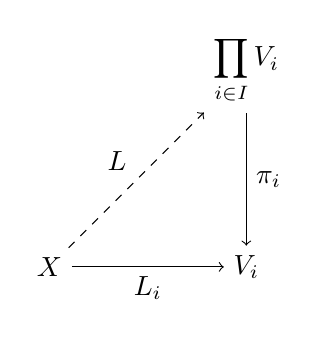
\begin{tikzpicture}[node distance=2.5cm, auto]
	\node (P) {$\displaystyle\prod_{i \in I} \bm{V_i}$};
	\node (Ci) [below of=P] {$\bm{V_i}$};
	\node (X) [left of=Ci] {$\bm X$};
	\draw[->] (X) to node [swap] {$L_i$} (Ci);
	\draw[->, dashed] (X) to node {$L$} (P);
	\draw[->] (P) to node {$\pi_i$} (Ci);
\end{tikzpicture}
\end{figure}
\end{proposition}
\begin{proof}
Defina a função
	\begin{align*}
	\func{L}{X}{\prod_{i \in I} V_i}{x}{(L_i(x))_{i \in I}}.
	\end{align*}
Da propriedade universal para conjuntos, $L$ é a única função de $X$ para $\bigtimes_{i \in I} \bm{V_i}$ tal que, para todo $i \in I$, $\pi_i \circ L = L_i$. Falta mostrar que $L$ é função linear. Sejam $c \in C$ e $x_1,x_2 \in V$. Então
	\begin{align*}
	L(x_1+cx_2) &= (L_i(x_1+cx_2))_{i \in I} \\
		&= (L_i(x_1)+cL_i(x_2))_{i \in I} \\
		&= (L_i(x_1))_{i \in I}+c(L_i(x_2))_{i \in I} \\
		&= L(x_1)+cL(x_2). \qedhere
	\end{align*}
\end{proof}

\subsection{Coproduto (soma)}

\begin{definition}
Seja $(\bm{V_i})_{i \in I} = ((V_i,+_i,\cdot_i))_{i \in I}$ uma família de espaços vetoriais. A \emph{soma categórica} de $(\bm{V_i})_{i \in I}$ é
	\begin{equation*}
	\coprod_{i \in I} \bm{V_i} = (V,+,\cdot),
	\end{equation*}
em que
	\begin{equation*}
	V = \set{v=(v_i)_{i \in I} \in \prod_{i \in I} V_i}{\card{\supp(v)} < \card{\N}},
	\end{equation*}
	\begin{align*}
	\func{+}{V \times V}{V}{(v,v')}{(v_i +_i {v'}_i)_{i \in I}}
	\end{align*}
e
	\begin{align*}
	\func{\cdot}{C \times V}{V}{(c,v)}{(cv_i)_{i \in I}.}
	\end{align*}
\end{definition}

Observe que, se $\card{I} < \card{\N}$, então $\prod_{i \in I} \bm{V_i} = \coprod_{i \in I} \bm{V_i}$.

\begin{proposition}[Propriedade Universal]
Sejam $(\bm{V_i})_{i \in I}$ uma família de espaços vetoriais sobre um corpo $\bm C$, $\bm X$ um espaço vetorial sobre $\bm C$ e, para todo $i \in I$, $L_i: \bm{V_i} \to \bm X$ uma função linear. Então existe única função linear $L: \bm X \to \coprod_{i \in I} \bm{V_i}$ tal que, para todo $i \in I$, $L \circ \iota_i = L_i$ (o diagrama comuta).
\begin{figure}
\centering
\begin{tikzpicture}[node distance=2.5cm, auto]
	\node (Ci) {$\bm{V_i}$};
	\node (S) [below of=Ci] {$\displaystyle\coprod_{i \in I} \bm{V_i}$};
	\node (X) [right of=Ci] {$\bm X$};
	\draw[->] (Ci) to node {$L_i$} (X);
	\draw[->, dashed] (S) to node [swap] {$L$} (X);
	\draw[->] (Ci) to node [swap] {$\iota_i$} (S);
\end{tikzpicture}
\end{figure}
\end{proposition}

O coproduto de espaços vetoriais é também chamado de \emph{soma} ou \emph{soma direta} e denotado
	\begin{equation*}
	\bigoplus_{i \in I} \bm{V_i}.
	\end{equation*}

%\cleardoublepage
%\section{Notas de Espaços Vetoriais Complexos}

%$(\C^m,i)$, sendo $i \cdot z:= (\sqrt{-1}z_1,\dots,\sqrt{-1}z_m)$.

%\begin{definition}
%Uma \emph{estrutura complexa} em $\R^{2m}$ é um mapa linear $j: \R^{2m} \to \R^{2m}$ que satisfaz
%	\begin{equation*}
%	j \circ j (v) = -v.
%	\end{equation*}
%\end{definition}
%
%Vamos definir uma ação de $\C$ em $\R^{2m}$.
%	\begin{equation*}
%	p(a+\sqrt{-1}b)(v) = av+bj(v).
%	\end{equation*}
%
%\begin{proposition}
%$(\R^{2m},j) \simeq (\C^m,i)$.
%\end{proposition}
%
%Para cada produto interno, temos um ângulo reto, logo uma multiplicação por $j$ distinta.
%
%Pode-se definir a partir de um vetor normal $n_p$ a um plano tangente em $p$ um mapa linear
%	\begin{equation*}
%	j_p(v) := v \times n_p
%	\end{equation*}
%que satisfaz ${j_p}^2 (v) = -v$.




\section{Projeções lineares}

\begin{definition}
Seja $\bm V$ um espaço linear sobre um corpo $\bm C$. Uma \emph{projeção linear} em $\bm V$ é uma função linear $p\colon V \to V$ idempotente: $p^2=p$.
\end{definition}

\begin{proposition}
Sejam $\bm V$ um espaço linear sobre um corpo $\bm C$ e $p\colon V \to V$ uma projeção linear.
	\begin{enumerate}
	\item $p|_{p(V)} = \Id|_{p(V)}$;
	
	\item $(\Id-p) \colon V \to V$ é uma projeção linear em $\bm V$;
	
	\item $(\Id-p)\inv(0) = p(V)$ e $(\Id-p)(V) = p\inv(0)$;
	
	\item $V = p(V) \oplus p\inv(0) = p(V) \oplus (\Id-p)(V)$;
	
	\item Para todo $\lambda \in C \setminus \{0,1\}$,
		\begin{equation*}
		(\lambda\Id-p)\inv = \frac{1}{\lambda}\Id + \frac{1}{\lambda(1-\lambda)}p
		\end{equation*}
portanto $\Esp(p) \subseteq \{0,1\}$;

	\item $p$ é invertível se, e somente se, $p=\Id$.

	\item Se $p \neq 0$, seu polinômio mínimo é $x^2-x = x(x-1)$, logo $p$ é diagonalizável pois tem raízes distintas.
	\end{enumerate}
\end{proposition}
\begin{proof}
	\begin{enumerate}	
	\item Seja $v \in p(V)$. Então existe $v' \in V$ tal que $v=p(v')$, logo
		\begin{equation*}
		p(v) = p(p(v')) = p^2(v') = p(v') = v.
		\end{equation*}
	
	\item A função $\Id-p$ é linear pois é uma diferença de funções lineares. Basta mostrar que ela é idempotente. Basta notar que% Para todo $v \in V$,
%		\begin{align*}
%		(\Id-p)^2(v) &= (\Id-p)(v-p(v)) \\
%			&= \Id(v-p(v)) - p(v-p(v)) \\
%			&= v-p(v)-p(v)+p^2(v) \\
%			&= v-p(v)-p(v)+p(v)\\
%			&= v-p(v)\\
%			&= (\Id-p)(v)
%		\end{align*}
%o que implica que $(\Id-p)^2 = \Id-p$.
		\begin{equation*}
		(\Id-p)^2 = \Id-p-p+p^2 = \Id-p-p+p = \Id-p.
		\end{equation*}
% INTERESSANTE poder multiplicar funções lineares assim, como se fosse a distributividade de multiplicação e adição. Provar isso generalizando depois.
	
	\item Seja $v \in (\Id-p)\inv(0)$. Então $(\Id-p)(v)=0$, logo $v=p(v)$, o que implica que $v \in p(V)$. Reciprocamente, seja $v \in p(V)$. Então do item 1 segue que $p(v) = v$, logo $(\Id-p)(v) = v-p(v) = v-v = 0$.

A outra relação segue de $(\Id-p)$ ser projeção e $p = \Id - (\Id-p)$.

	\item Seja $v \in p(V) \cap p\inv(0)$. Então $p(v)=0$ e $p(v)=v$, o que implica que $v = p(v) = 0$. Assim temos que $p(V) \cap p\inv(0) = \{0\}$.
%Sejam $v in p(V)$ e $v' \in p\inv(0)$ e $c,c' \in C$ tais que $cv+c'v'=0$. Então
%		\begin{equation*}
%		0 = p(0) = p(cv+c'v') = cp(v)+c'p(v') = cv
%		\end{equation*}
%logo $c=0$, portanto $0 = cv+c'v'=c'v'$, o que implica que $c'=0$.
	
	Seja $v \in V$. Então $p(v) \in p(V)$ e $(\Id-p)(v) \in p\inv(0)$ (pois $(\Id-p)(V) = p\inv(0)$), logo $v = p(v) + (\Id-p)(v)$, o que mostra que $V = p(V) + p\inv(V)$.
	
	\item Note que
		\begin{equation*}
		\frac{1}{1-\lambda} - \frac{1}{\lambda} - \frac{1}{\lambda(1-\lambda)} = \frac{\lambda - (\lambda - 1) - 1}{\lambda(1-\lambda)} = 0,
		\end{equation*}
logo
		\begin{align*}
		(\lambda\Id - p) \circ \left( \frac{1}{\lambda}\Id + \frac{1}{\lambda(1-\lambda)}p \right) &= \Id + \frac{1}{1-\lambda}p - \frac{1}{\lambda}p - \frac{1}{\lambda(1-\lambda)}p^2 \\
%			&= \Id + \frac{1}{1-\lambda}p - \frac{1}{\lambda}p - \frac{1}{\lambda(1-\lambda)}p \\
			&= \Id + \left( \frac{1}{1-\lambda} - \frac{1}{\lambda} - \frac{1}{\lambda(1-\lambda)} \right) p \\
			&= \Id.
		\end{align*}
e
	\begin{equation*}
	\left( \frac{1}{\lambda}\Id + \frac{1}{\lambda(1-\lambda)}p \right) \circ (\lambda\Id - p) = \Id - \frac{1}{\lambda}p + \frac{1}{1-\lambda}p - \frac{1}{\lambda(1-\lambda)}p^2 = \Id.
	\end{equation*}
	
	\item Se $p$ é invertível, $V=p(V)$, logo
		\begin{equation*}
		p = p|_{V} = p|_{p(V)} = \Id|_{p(V)} = \Id|_V = \Id.
		\end{equation*}
A recíproca é evidente.

	\item Evidente.
	
	\end{enumerate}
\end{proof}




%\chapter{Álgebra Multilinear}

\section{Funções multilineares}

\begin{definition}
Sejam $\bm{V_0},\cdots,\bm{V_{k-1}}$ e $\bm W$ espaços lineares sobre um corpo $\bm C$ e $k \in \N$. Uma função \emph{$k$-linear} de $(\bm{V_0},\ldots,\bm{V_{k-1}})$ para $\bm W$ é uma função
	\begin{equation*}
	L\colon V_0 \times \cdots \times V_{k-1} \to W
	\end{equation*}
qua satisfaz
	\begin{enumerate}
	\item (Multilinearidade) Para todos $i \in [k]$ e
	\begin{equation*}
	(v_0,\ldots,v_{i-1},v_{i+1},\ldots,v_{k-1}) \in V_0 \times \cdots \times V_{i-1} \times V_{i+1} \times \cdots \times V_{k-1},
	\end{equation*}
a função
	\begin{align*}
	\func{L(v_0,\ldots,v_{i-1},\var,v_{i+1},\ldots,v_{k-1})}{\bm{V_i}}{\bm W}{v}{L(v_0,\ldots,v_{i-1},v,v_{i+1},\ldots,v_{k-1})}
	\end{align*}
%	\begin{align*}
%	\func{L(\bm v_0,\ldots,\underbrace{\var}_i,\ldots,\bm v_{k-1})}{\bm{V_i}}{\bm W}{\bm v}{L(\bm v_0,\ldots,\underbrace{\bm v}_i,\ldots,\bm v_{k-1})}
%	\end{align*}
é uma função linear.
	\end{enumerate}
O conjunto dessas funções é denotado
	\begin{equation*}
	\lin(V_0,\ldots,V_{k-1};W)
	\end{equation*}
e, quando todos os espaços $\bm{V_i}$ são iguais, denota-se
	\begin{equation*}
	\lin^k(V,W) := \lin(\underbrace{V,\ldots,V}_k;W)
	\end{equation*}
\end{definition}

\begin{proposition}
Sejam $\bm{V_0},\cdots,\bm{V_{k-1}}$ e $\bm W$ espaços lineares sobre um corpo $\bm C$ e, para cada $i \in [k]$, $d_i \in \N$ a dimensão e $b^{(i)}=(b^{(i)}_j)_{j \in [d_i]}$ uma base ordenada de $\bm{V_i}$. Toda função $k$-linear $L \in \lin(V_0,\ldots,V_{k-1};W)$ está determinada pelos seus valores em $(b^{(0)}_{j_0},\ldots,b^{(k-1)}_{j_{k-1}})_{(j_0,\ldots,j_{k-1}) \in [d_0] \times \cdots \times [d_{k-1}]}$.
\end{proposition}
\begin{proof}
Sejam $v_0,\ldots,v_{m-1} \in V_k$, $c^0,\ldots,c^{m-1} \in C$, e, para todo $i \in [k]\setminus \{k\}$, $v'_i \in V_i$. Como consequência da propriedade de linearidade generalizada para funções lineares,
	\begin{equation*}
	L\left(v'_0,\ldots,\sum_{i \in [m]} c^i v_i,\ldots,v'_{k-1} \right) = \sum_{i \in [m]} c^i L\left(v'_0,\ldots,v_i,\ldots,v'_{k-1} \right).
	\end{equation*}
Sendo assim, para cada $i \in [k]$, sejam $v_i \in V_i$ e $v_{(i)}^0,\ldots,v_{(i)}^{d_i} \in C$ os coeficientes de $v_i$ na base $b^{(i)}$, de modo que
	\begin{equation*}
	v_i = \sum_{j \in [d_i]} v_{(i)}^j b^{(i)}_j.
	\end{equation*}
Pela linearidade em cada entrada, temos que
	\begin{align*}
	L(v_0,\ldots,v_{k-1}) &= L\left(\sum_{j_0 \in [d_0]} v_{(0)}^{j_0}b^{(0)}_{j_0},\ldots,\sum_{j_{k-1} \in [d_{k-1}]} v_{(k-1)}^{j_{k-1}} b^{(k-1)}_{j_{k-1}} \right) \\
		&= \sum_{j_0 \in [d_0]} v_{(0)}^{j_0} L\left(b^{(0)}_{j_0},\ldots,\sum_{j_{k-1} \in [d_{k-1}]} v_{(k-1)}^{j_{k-1}} b^{(k-1)}_{j_{k-1}} \right) \\
		&\ \, \vdots\qquad\qquad\qquad\qquad\qquad \vdots \\
		&= \sum_{j_0 \in [d_0]} \cdots \sum_{j_{k-1} \in [d_{k-1}]} v_{(0)}^{j_0} \cdots v_{(k-1)}^{j_{k-1}} L\left(b^{(0)}_{j_0},\ldots,b^{(k-1)}_{j_{k-1}} \right) \\
		&= \sum_{(j_0,\ldots,j_{k-1}) \in [d_0] \times \cdots \times [d_{k-1}]} v_{(0)}^{j_0} \cdots v_{(k-1)}^{j_{k-1}} L\left(b^{(0)}_{j_0},\ldots,b^{(k-1)}_{j_{k-1}} \right).
	\end{align*}
%			&= \sum_{\substack{j_0 \in [d_0] \\ \cdots\\ j_{k-1} \in [d_{k-1}]}} v_{0,j_0} \cdots v_{k-1,j_{k-1}} L\left(b_{0,j_0},\ldots,b_{k-1,j_{k-1}} \right).
Portanto a função $L$ está determinada pelos valores que tem nos elementos
	\begin{equation*}
	(b^{(0)}_{j_0},\ldots,b^{(k-1)}_{j_{k-1}})_{(j_0,\ldots,j_{k-1}) \in [d_0] \times \cdots \times [d_{k-1}]}.
	\end{equation*}
%Como há $d_0 \cdots d_{k-1}$ desses elementos, há essa quantidade de escolhas a serem determinadas para se determinarem os valores de $L$.
\end{proof}

\begin{proposition}
Sejam $\bm{V_0},\cdots,\bm{V_{k-1}}$ e $\bm W$ espaços lineares sobre um corpo $\bm C$. Então
	\begin{equation*}
	\lin(\bm{V_0},\ldots,\bm{V_{k-1}};\bm W) := (\lin(V_0,\ldots,V_{k-1};W),+,\cdot),
	\end{equation*}	
em que $+$ e $\cdot$ são a soma e o produto escalar pontuais induzidos por $\bm W$, é um espaço linear sobre $\bm C$.
\end{proposition}

%Mostrar isomorfismo
%	\begin{align*}
%	\func{\Omega}{\lin^2(V_0,V_1;W)}{\lin(V_0,\lin(V_1,W))}{L}{L(v_0,\var)}.
%	\end{align*}

\subsection{Simetria, antissimetria e alternância}

\begin{definition}
Sejam $\bm V$ e $\bm W$ espaços lineares sobre um corpo $\bm C$. Uma função $k$-linear de $\bm V$ para $\bm W$
\begin{enumerate}
	\item \emph{simétrica} é uma função $f \in \lin^k(\bm V,\bm W)$ tal que, para toda permutação $p \in \sime_k$ e todos $v_0$, $\ldots$, $v_{k-1} \in V$,
	\begin{equation*}
	f(v_{p(0)},\ldots,v_{p(k-1)}) = f(v_0,\ldots,v_{k-1});
	\end{equation*}
O conjunto das funções $k$-lineares simétricas é denotado $\mathcal S^k(\bm V,\bm W)$.
	\item \emph{antissimétrica} é uma função $f \in \lin^k(\bm V,\bm W)$ tal que, para toda permutação $p \in \sime_k$ e todos $v_0,\ldots,v_{k-1} \in V$,
	\begin{equation*}
	f(v_{p(0)},\ldots,v_{p(k-1)}) = \prd(p) f(v_0,\ldots,v_{k-1});
	\end{equation*}
	\item \emph{alternada} é uma função $f \in \lin^k(\bm V,\bm W)$ tal que, para todos $v_0,\ldots,v_{k-1} \in V$ linearmente dependentes,
	\begin{equation*}
	f(v_0,\ldots,v_{k-1}) = 0.
	\end{equation*}
O conjunto das funções $k$-lineares alternadas é denotado $\mathcal A^k(\bm V,\bm W)$.
\end{enumerate}
\end{definition}

\begin{proposition}
Sejam $\bm V$ e $\bm W$ espaços lineares sobre um corpo $\bm C$ e $f \in \lin^k(\bm V,\bm W)$.
	\begin{enumerate}
	\item A função $f$ é alternada se, e somente se, para todos $v_0$, $\ldots$, $v_{k-1} \in V$ tais que existem $i,j \in [k]$ distintos satisfazendo $v_i = v_j$,
	\begin{equation*}
	f(v_0,\ldots,v_{k-1})=0.
	\end{equation*} 
	\item Se $f$ é alternada, então é antissimétrica. Se $\car(\bm C) \neq 2$ e $f$ é antissimétrica, então é alternada.
	\item Se $\car(\bm C) = 2$, então $f$ é antissimétrica se, e somente se, é simétrica.
	\end{enumerate}
\end{proposition}
\begin{proof}
	\begin{enumerate}
	\item Se $f$ é alternada, então, para todos $v_0,\ldots,v_{k-1} \in V$ tais que $v_i = v_j$ para dois $i,j \in [k]$ distintos, o conjunto $\{v_0,\ldots,v_{k-1}\}$ é linearmente dependente, portanto $f(v_0,\ldots,v_{k-1})=0$. Reciprocamente, suponha que $f$ satisfaz a propriedade e sejam $v_0,\ldots,v_{k-1} \in V$ linearmente dependentes. Então existe $i \in [k]$ tal que $v_i$ é combinação linear dos outros $v_j$: existem $c_j \in C$, com $j \in [k]\setminus\{i\}$, tais que
	\begin{equation*}
	v_i = \sum_{j \in [k]\setminus\{i\}} c_j v_j.
	\end{equation*}
Assim, segue da $k$-linearidade e da propriedade enunciada que
	\begin{align*}
	f(v_0,\ldots,v_{k-1}) &= f\left(v_0,\ldots, \sum_{j \in [k]\setminus\{i\}} c_j v_j,\ldots,v_{k-1}\right) \\
		&= \sum_{j \in [k]\setminus\{i\}} c_j f(v_0,\ldots,v_j,\ldots,v_{k-1}) \\
		&=\sum_{j \in [k]\setminus\{i\}} c_j 0 = 0.
	\end{align*}

	\item Suponha $f$ alternada e sejam $v_0,\ldots,v_{k-1} \in V$. Então segue da $k$-linearidade e da alternância de $f$ que
	\begin{align*}
	0 =&f(v_0,\ldots,v_i+v_j,\ldots,v_i+v_j,\ldots,v_{k-1}) \\
		=& f(v_0,\ldots,v_i,\ldots,v_i,\ldots,v_{k-1}) + f(v_0,\ldots,v_i,\ldots,v_j,\ldots,v_{k-1}) \\
		&+f(v_0,\ldots,v_j,\ldots,v_i,\ldots,v_{k-1}) + f(v_0,\ldots,v_j,\ldots,v_j,\ldots,v_{k-1}) \\
		=& f(v_0,\ldots,v_i,\ldots,v_j,\ldots,v_{k-1}) +f(v_0,\ldots,v_j,\ldots,v_i,\ldots,v_{k-1}),
	\end{align*}
portanto
	\begin{equation*}
	f(v_0,\ldots,v_i,\ldots,v_j,\ldots,v_{k-1}) = - f(v_0,\ldots,v_j,\ldots,v_i,\ldots,v_{k-1}).
	\end{equation*}
Como toda permutação $p \in \sime_k$ é um produto de $N \in \N$ inversões, e como $\prd(p)=(-1)^N$, segue por indução que, para toda permutação $p \in \sime_k$,
	\begin{equation*}
	f(v_{p(0)},\ldots,v_{p(k-1)}) =(-1)^N f(v_0,\ldots,v_{k-1}) = \prd(p) f(v_0,\ldots,v_{k-1}).
	\end{equation*}

Suponha que $\car(\bm C) \neq 2$. Sejam $f \in \lin^k(\bm V,\bm W)$ antissimétrica e $v_0$, $\ldots$, $v_{k-1} \in V$ tais que $v_i = v_j$ para dois $i,j \in [k]$ distintos. Considerando a permutação $(i \quad j) \in \sime_k$, segue da antissimetria de $f$ e de $\prd((i \quad j))=-1$ que
	\begin{align*}
	f(v_0,\ldots,v_i,\ldots,v_j,\ldots,v_{k-1}) &= f(v_0,\ldots,v_j,\ldots,v_i,\ldots,v_{k-1}) \\
		&= - f(v_0,\ldots,v_i,\ldots,v_j,\ldots,v_{k-1}),
	\end{align*}
portanto
	\begin{equation*}
	2 f(v_0,\ldots,v_{k-1})=0.
	\end{equation*}
Como $\car(\bm C) \neq 2$, segue que $f(v_0,\ldots,v_{k-1})=0$. Do item 1 segue que $f$ é alternada.

\item Se $\car(\bm C) = 2$, então $-1=1$. Isso implica que, para qualquer permutação $p$, $\prd(p)=1$.
\end{enumerate}
\end{proof}

Um exemplo de uma função multilinear que é antissimétrica mas não é alternada em para um corpo de característica $2$ é o seguinte. Seja $\Z_2=\{0,1\}$ o corpo de característica $2$ e considere a função $f\colon \Z_2 \times \Z_2 \to \Z_2$ dada por
	\begin{align*}
	\func{f}{\Z_2 \times \Z_2}{\Z_2}{(0,0)}{0 \\
															(0,1) &\mapsto 0 \\
															(1,0) &\mapsto 0 \\
															(1,1) &\mapsto 1												
														}
	\end{align*}
Pode-se verificar que essa função é bilinear e antissimétrica, mas não é alternada porque $f(1,1)=1 \neq 0$.

De modo mais geral, para qualquer função $p\colon [k] \to [k]$, não necessariamente bijetiva, considerando o caráter $\prd(p)$ que vale $0$ se $p$ não é uma permutação, e $1$ ou $-1$ conforme a paridade da permutação $p$, as definições de formas antissimétricas e alternadas podem ser unificadas: a de formas antissimétricas pode ser mantida como foi feita e, para o caso de formas alternadas, devido à propriedade 1 da proposição anterior, pode-se enunciar: para qualquer $p\colon [k] \to [k]$,
	\begin{equation*}
	f(v_{p(0)},\ldots,v_{v_{k-1}}) = \prd(p) f(v_0,\ldots,v_{k-1}).
	\end{equation*}
O caso em que $p$ é bijetiva recai na definição de formas antissimétricas, e o caso em que $p$ não é bijetiva recai na definição de formas alternadas, mais precisamente da propriedade 1 da proposição anterior, que é equivalente à definição de forma alternada.

\begin{proposition}
Sejam $\bm V$ e $\bm W$ espaços lineares sobre um corpo $\bm C$. Os espaços $\mathcal S^k(\bm V,\bm W)$ e $\mathcal A^k(\bm V,\bm W)$ são subespaços lineares de $\lin^k(\bm V,\bm W)$.
\end{proposition}


\subsection{Espaços de funções multilineares}

\begin{proposition}
\label{prop:isomorfismo.espacolinear.espacobilinear}
Sejam $\bm V$ e $\bm V'$ e $\bm V''$ espaços lineares sobre um corpo $\bm C$. Os espaços são linearmente isomorfos.
	\begin{equation*}
	\lin(\bm V,\lin(\bm V',\bm V'')) \simeq \lin(\bm V,\bm V';\bm V'').
	\end{equation*}
\end{proposition}
\begin{proof}
Denotaremos uma função $f \in \lin(\bm V,\lin(\bm V',\bm V''))$ por
	\begin{align*}
	\func{f}{V}{\lin(\bm V',\bm V'')}{v}{
		\begin{aligned}[t]
		\func{f_v}{V'}{V''}{v'}{f_v(v')}.
		\end{aligned}
	}
	\end{align*}
Definimos as funções
	\begin{align*}
	\func{I}{\lin(\bm V,\lin(\bm V',\bm V''))}{\lin(\bm V,\bm V';\bm V'')}{f}{
		\begin{aligned}[t]
		\func{I(f)}{V \times V'}{V''}{(v,v')}{f_v(v')}
		\end{aligned}
	}
	\end{align*}
e
	\begin{align*}
	\func{J}{\lin(\bm V,\bm V';\bm V'')}{\lin(\bm V,\lin(\bm V',\bm V''))}{f}{
		\begin{aligned}[t]
		\func{J(f)}{V}{\lin(\bm V',\bm V'')}{v}{
			\begin{aligned}[t]
			\func{J(f)_v}{V'}{V''}{v'}{f(v,v')}.
			\end{aligned}
		}
		\end{aligned}
	}
	\end{align*}
É simples mostrar que $I$ e $J$ estão bem definidas, são lineares e uma é inversa da outra.
\end{proof}




\section{Formas multilineares}

\begin{definition}
Seja $\bm V$ um espaço linear sobre um corpo $\bm C$. Uma \emph{forma $k$-linear} em $\bm V$ é uma função $f \in \lin^k(\bm V;\bm C)$, ou seja, um funcional $k$-linear em $(\bm V,\ldots,\bm V)$. O conjunto das formas $k$-lineares simétricas é denotado $\mathcal{S}^k(\bm V)$ e o das alternadas é denotado $\mathcal{A}^k(\bm V)$.
\end{definition}

Temos que $\mathcal{S}^1(\bm V) = \mathcal{A}^1(\bm V) = \lin^k(\bm V)$ e $\mathcal{S}^0(\bm V) = \mathcal{A}^0(\bm V) = \lin^0(\bm V) = C$.

\subsection{Produto tensorial de formas multilineares}

\begin{definition}
Sejam $\bm V$ um espaço linear sobre um corpo $\bm C$, $f \in \lin^k(V)$, $f' \in \lin^{k'}(V)$ e $v_0,\ldots,v_{k+k'-1} \in V$. O \emph{produto tensorial} de $f$ e $f'$ em $(v_0,\ldots,v_{k+k'-1})$ é
	\begin{equation*}
	(f \otimes f')(v_0,\ldots,v_{k+k'-1}) := f(v_0,\ldots,v_{k-1})f'(v_k,\ldots,v_{k+k'-1}).
	\end{equation*}
Sejam $n \in \N$ e $(f_i)_{i \in [n]}$ formas multilineares em $\bm V$. O \emph{produto tensorial} dessas formas é definido recursivamente
	\begin{equation*}
	\bigotimes_{i \in [n]} f_i := \begin{cases}
		f_0,& n=1 \\
		\left(\displaystyle\bigotimes_{i \in [n-1]} f_i \right) \otimes f_{n-1} ,& n>1.
	\end{cases}
	\end{equation*}
\end{definition}

\begin{proposition}
Seja $\bm V$ um espaço linear sobre um corpo $\bm C$.
	\begin{enumerate}
	\item Para todas formas $f \in \lin^k(\bm V)$ e $f' \in \lin^{k'}(\bm V)$, a função $f \otimes f'$ é uma forma $k+k'$-linear.
	\item (Bilinearidade) A função
		\begin{align*}
		\func{\otimes}{\lin^k(\bm V) \times \lin^{k'}(\bm V)}{\lin^{k+k'}(\bm V)}{(f,f')}{f \otimes f'}
		\end{align*}
é bilinear.
	\item (Associatividade) Para todas formas $f \in \lin^k(\bm V)$, $f' \in \lin^{k'}(\bm V)$ e $f'' \in \lin^{k''}(\bm V)$,
		\begin{equation*}
		(f \otimes f') \otimes f'' = f \otimes (f' \otimes f'').
		\end{equation*}
	\end{enumerate}
\end{proposition}

\subsection{Produto alternado de formas multilineares}

\begin{definition}
Sejam $\bm V$ um espaço linear sobre um corpo $\bm C$, $f \in \mathcal{A}^k(\bm V)$, $f' \in \mathcal{A}^{k'}(\bm V)$ e $v_0,\ldots,v_{k+k'-1} \in \bm V$. O \emph{produto alternado} (ou \emph{exterior}) de $f$ e $f'$ em $(v_0,\ldots,v_{k+k'-1})$ é
%	\begin{equation*}
%	(f \wedge f')(v_0,\ldots,v_{k+k'-1}) := \frac{1}{k!k'!} \sum_{p \in \sime_{k+k'}} \prd(p) f(v_{p(0)},\ldots,v_{p(k-1)})f'(v_{p(k)},\ldots,v_{p(k+k'-1)}).
%	\end{equation*}
	\begin{equation*}
	(f \wedge f')(v_0,\ldots,v_{k+k'-1}) := \frac{1}{k!k'!} \sum_{p \in \sime_{k+k'}} \prd(p) (f \otimes f')(v_{p(i)})_{i \in [k+k']}.
	\end{equation*}
Sejam $n \in \N$ e $(f_i)_{i \in [n]}$ formas multilineares em $\bm V$. O \emph{produto alternado} dessas formas é definido recursivamente
	\begin{equation*}
	\bigwedge_{i \in [n]} f_i := \begin{cases}
		f_0,& n=1 \\
		\left(\displaystyle\bigwedge_{i \in [n-1]} f_i \right) \wedge f_{n-1} ,& n>1.
	\end{cases}
	\end{equation*}
\end{definition}

\begin{proposition}
Seja $\bm V$ um espaço linear sobre um corpo $\bm C$.
	\begin{enumerate}
	\item Para todas formas $f \in \lin^k(\bm V)$ e $f' \in \lin^{k'}(\bm V)$, a função $f \wedge f'$ é uma forma $k+k'$-linear alternada.
	\item (Bilinearidade) A função
		\begin{align*}
		\func{\wedge}{\mathcal{A}^k(\bm V) \times \mathcal{A}^{k'}(\bm V)}{\mathcal{A}^{k+k'}(\bm V)}{(f,f')}{f \wedge f'}
		\end{align*}
é bilinear.
	\item (Associatividade) Para todas formas alternadas $f \in \mathcal{A}^k(\bm V)$, $f' \in \mathcal{A}^{k'}(\bm V)$ e $f'' \in \mathcal{A}^{k''}(\bm V)$,
		\begin{equation*}
		(f \wedge f') \wedge f'' = f \wedge (f' \wedge f'').
		\end{equation*}
	\item	 Para todas formas $f \in \mathcal{A}^k(\bm V)$ e $f' \in \mathcal{A}^{k'}(\bm V)$
		\begin{equation*}
		f' \wedge f = (-1)^{kk'} f \wedge f'.
		\end{equation*}
	\end{enumerate}
\end{proposition}
\begin{proof}
	\begin{enumerate}
	\item Seja $v_0,\ldots,v_{k+k'-1} \in V$ e $\bar p \in \sime_{k+k'}$. Então
		\begin{align*}
		(f \wedge f') (v_{\bar p(i)})_{i \in [k+k']} &= \frac{1}{k!k'!} \sum_{p \in \sime_{k+k'}} \prd(p) (f \otimes f')(v_{p(\bar p(i))})_{i \in [k+k']} \\
			&= \frac{1}{k!k'!} \sum_{p \in \sime_{k+k'}} \prd(\bar p\inv p) (f \otimes f')(v_{p(i)})_{i \in [k+k']} \\
			&= \frac{1}{k!k'!} \sum_{p \in \sime_{k+k'}} \prd(\bar p\inv)\prd(p) (f \otimes f')(v_{p(i)})_{i \in [k+k']} \\
			&= \prd(\bar p\inv)\frac{1}{k!k'!} \sum_{p \in \sime_{k+k'}} \prd(p) (f \otimes f')(v_{p(i)})_{i \in [k+k']} \\
			&= \prd(\bar p)(f \wedge f')(v_i)_{i \in [k+k']}.
		\end{align*}
	\item	 
	\end{enumerate}
\end{proof}

%Isso define uma função bilinear
%	\begin{align*}
%	\func{\wedge}{\mathcal{A}^k(\bm V) \times \mathcal{A}^l(\bm V)}{\mathcal{A}^{k+l}(\bm V)}{(f,g)}{f \wedge g}
%	\end{align*}

%Esse produto é uma forma $\sum_{i \in [n]} k_i$-linear em $\bm V$.

%\begin{definition}
%Sejam $\bm V$ um espaço linear de dimensão finita $d$ sobre um corpo $\bm C$, $(b_i)_{i \in [d]}$ um base ordenada de $\bm V$ e $({b_i}^*)_{i \in [d]}$ a base dual de $\bm{V^*}$. Para todo subconjunto $I \subseteq [d]$, e $(i_j)_{j \in [\card{I}]}$ a indexação crescente de $I$ ($i_0 < \cdots < i_{\card{I}-1}$), define-se
%	\begin{equation*}
%	\bigwedge_{i \in I} b_i^* := b_{i_0}^* \wedge \cdots \wedge b_{i_{k-1}}^*.
%	\end{equation*}
%\end{definition}

\begin{proposition}
Sejam $\bm V$ um espaço linear de dimensão finita $d$ sobre um corpo $\bm C$, $(b_i)_{i \in [d]}$ um base ordenada de $\bm V$ e $({b_i}^*)_{i \in [d]}$ a base dual de $\bm{V^*}$. Então $\mathcal{A}^k(\bm V)$ é um espaço linear sobre $\bm C$ de dimensão $\binom{d}{k}$ e o conjunto
	\begin{equation*}
	\set{b_{i_0}^* \wedge \cdots \wedge b_{i_{k-1}}^*}{i_0 < \cdots < i_{k-1} \in [d]}
	\end{equation*}
%	\begin{equation*}
%	\set{\bigwedge_{i \in I} b_{i}^*}{I \subseteq [d], \card{I}=k}
%	\end{equation*}
de formas alternadas $k$-lineares em $\bm V$ é uma base para $\mathcal{A}^k(\bm V)$.
\end{proposition}

Em particular, isso mostra que formas $d$-lineares num espaço de dimensão $d$ são todas múltiplos umas das outras, pois $\binom{d}{d}=1$. Podemos fixar o valor de uma das formas como 1 na base canônica e chamá-la de \emph{determinante}.

\begin{definition}
Seja $d \in \N$. O \emph{determinante} em $\R^d$ é a forma $d$-linear
	\begin{equation*}
	\det{\var,\cdots,\var} := {\ii_0}\dual \wedge \ldots \wedge {\ii_{d-1}}\dual.
	\end{equation*}
%Sejam $\bm V$ um espaço linear de dimensão finita $d$ sobre um corpo $\bm C$ e $b=(b_i)_{i \in [d]}$ uma base de $\bm V$. O \emph{determinante} em $\bm V$ com respeito a $b$ é a forma $d$-linear
%	\begin{equation*}
%	\det{\var,\cdots,\var}\nolimits_{b} := {b_0}\dual \wedge \ldots \wedge {b_{d-1}}\dual.
%	\end{equation*}
%No caso de $V = \R^d$, o determinante é definido com respeito à base canônica
%	\begin{equation*}
%	\det{\var,\cdots,\var} := {\ii_0}\dual \wedge \ldots \wedge {\ii_{d-1}}\dual.
%	\end{equation*}
\end{definition}

Como comentado, essa é a única forma $d$-linear em $\R^d$ tal que	\begin{equation*}
	\det{\ii_0,\ldots,\ii_{d-1}}=1.
	\end{equation*}

Na seção seguinte, definiremos o conceito de determinante de modo mais geral e independente de base.

\subsection{Formas puxadas e determinante}

\begin{definition}
Sejam $\bm V$ e $\bm V'$ espaços lineares sobre um corpo $\bm C$, $L \colon V \to V'$ uma função linear e $f \in \lin^k(V')$. A \emph{forma $k$-linear puxada} por $L$ de $f$ é a função
	\begin{align*}
	\func{L\dual f}{V^k}{C}{(v_0,\ldots,v_{k-1})}{f(L(v_0),\ldots,L(v_{k-1})).}
	\end{align*}
A função \emph{$k$-adjunta} induzida por $L$ é a função linear
	\begin{align*}
	\func{L\dual}{\lin^k(V')}{\lin^k(V)}{f}{L\dual f.}
	\end{align*}
\end{definition}

A notação é ambígua porque, para cada $k \in [d+1]$, a função $L\dual$ é uma função diferente. De fato, para $f \in \lin^k(V')$,
	\begin{equation*}
	L\dual f = f \circ L^{\otimes k},
	\end{equation*}
o que quer dizer que
	\begin{equation*}
	L \dual = (L^{\otimes k})\pux
	\end{equation*}

\begin{proposition}
Sejam $\bm V$, $\bm V'$ e $\bm V''$ espaços lineares sobre um corpo $\bm C$ e $L\colon V \to V'$ e $L'\colon V' \to V''$ funções lineares. Então
	\begin{equation*}
	(L' \circ L)\dual = {L}\dual \circ {L'}\dual.
	\end{equation*}
\end{proposition}
\begin{proof} Seja $f \in \lin^k(V)$ tal que $f \neq 0$. Então
	\begin{align*}
	(L' \circ L)\dual f (v_0,\ldots,v_{k-1}) &= f((L' \circ L)(v_0),\ldots,(L' \circ L)(v_{k-1})) \\
		&= f(L'(L(v_0)),\ldots,L'(L(v_{k-1}))) \\
		&= {L'}\dual f(L(v_0),\ldots,L(v_{k-1})) \\
		&= L\dual({L'}\dual f)(v_0,\ldots,v_{k-1}) \\
		&= (L\dual \circ {L'}\dual) f(v_0,\ldots,v_{k-1}).
	\end{align*}
\end{proof}


Essas funções $k$-adjuntas estão também definidas se restringimos os espaços de funcionais $\lin^k$ para espaços de funcionais alternados $\alter^k$. Se considerarmos um espaço linear $d$-dimensional $\bm V$, o espaço $\alter^d(\bm V)$ é um espaço $1$-dimensional, o que implica que todas funções lineares são multiplicações por escalares. Isso nos permite definir o determinante de uma função linear intrinsecamente como o escalar que representa seu $d$-adjunto.

\begin{definition}
Sejam $\bm V$ um espaço linear $d$-dimensional sobre um um corpo $\bm C$, $L\colon V \to V$ uma função linear e $L\dual\colon \alter^d(V) \to \alter^d(V)$. O \emph{determinante} de $L$ é o escalar $\det{L} \in C$ tal que, para toda forma $f \in \alter^d(\bm V)$,
	\begin{equation*}
	L\dual f = \det{L} f.
	\end{equation*}
\end{definition}

Isso nos dá por definição a igualdade
	\begin{equation*}
	f(L(v_0),\ldots,L(v_{d-1})) = \det{L}f(v_0,\ldots,v_{d-1}).
	\end{equation*}

\begin{proposition}
Sejam $\bm V$ um espaço linear $d$-dimensional sobre um um corpo $\bm C$ e $L,L' \in \lin(V,V)$. Então
	\begin{equation*}
	\det{L' \circ L} = \det{L}\det{L'}.
	\end{equation*}
\end{proposition}
\begin{proof}
Seja $f \in \alter^n(V)$ tal que $f \neq 0$. Então
	\begin{equation*}
	\det{L' \circ L}f = (L' \circ L)\dual f = ({L}\dual \circ {L'}\dual) f = \det{L}\det{L'} f.
	\end{equation*}
\end{proof}

\begin{proposition}
Sejam $\bm V$ um espaço linear $d$-dimensional sobre um um corpo $\bm C$ e $L\colon V \to V$ uma função linear. Então $L$ é invertível se, e somente se, $\det{L} \neq 0$.
\end{proposition}
\begin{proof}
Basta notar que $L$ é invertível se, e somente se, leva base em base e $f \in \alter^d(V)$ é nula em um conjunto linearmente independente de vetores.
\end{proof}




\subsection{Formas bilineares simétricas e formas quadráticas}

\begin{definition}
Seja $\bm V$ um espaço linear sobre um corpo $\bm C$. Uma \emph{forma quadrática} em $\bm V$ é uma função $\fun{\qua{\var}}{V}{C}$ que satisfaz
	\begin{enumerate}
	\item ($2$-Homogeneidade) Para todos $c \in C$ e $v \in V$, $\qua{cv} = c^2 \qua{v}$;
	\item (Bilinearidade polar) A função
		\begin{align*}
		\func{b}{V \times V}{C}{(v,v')}{\qua{v+v'} - \qua{v} - \qua{v'}}
		\end{align*}
	é uma forma bilinear.
	\end{enumerate}
Um \emph{espaço quadrático} é um par $(\bm V,\qua{\var})$ em que $\bm V$ é um espaço linear (de dimensão finita) e $\qua{\var}$ uma forma quadrática em $\bm V$.
\end{definition}

\begin{proposition}
Seja $\bm V$ um espaço linear sobre um corpo $\bm C$ de característica diferente de $2$.
	\begin{enumerate}
	\item Se $\qua{\var}$ uma forma quadrática em $\bm V$, a função
		\begin{align*}
		\func{\inte{\var}{\var}}{V \times V}{C}{(v,v')}{\frac{\qua{v+v'} - \qua{v} - \qua{v'}}{2}}
		\end{align*}
	é uma $2$-forma simétrica e, para todo $v \in V$, $\qua{v} = \inte{v}{v}$.
	\item Se ${\inte{\var}{\var}}$ uma $2$-forma simétrica em $\bm V$. A função
		\begin{align*}
		\func{\qua{\var}}{V}{C}{v}{\inte{v}{v}}
		\end{align*}
	é uma forma quadrática e, para todos $v,v' \in V$, $\inte{v}{v'} = \frac{\qua{v+v'} - \qua{v} - \qua{v'}}{2}$.
	\end{enumerate}
\end{proposition}
\begin{proof}
	\begin{enumerate}
	\item Primeiro mostramos que $\inte{\var}{\var}$ é bilinear simétrica.
		\begin{itemize}
		\item (Bilinearidade) Segue da bilinearidade de $b(v,v') = \qua{v+v'} - \qua{v} - \qua{v'}$ que $\inte{\var}{\var} = \frac{1}{2}b$ é bilinear.
		\item (Simetria) Para todos $v,v' \in V$,
			\begin{align*}
			\inte{v}{v'} = \frac{\qua{v+v'} - \qua{v} - \qua{v'}}{2} = \frac{\qua{v'+v} - \qua{v'} - \qua{v}}{2} = \inte{v'}{v}.
			\end{align*}
		\end{itemize}
	Por fim, segue da $2$-homogeneidade de $\qua{\var}$ que, para todo $v \in V$,
		\begin{align*}
		\inte{v}{v} &= \frac{\qua{v+v} - \qua{v} - \qua{v}}{2} \\
			&= \frac{\qua{2v} - 2\qua{v}}{2} \\
			&= \frac{4\qua{v} - 2\qua{v}}{2} \\
			&= \frac{2\qua{v}}{2} \\
			&= \qua{v}.
		\end{align*}
	
	\item Primeiro mostramos que $\qua{\var}$ é forma quadrática.
		\begin{itemize}
			\item ($2$-Homogeneidade) Para todos $c \in C$ e $v \in V$, segue da bilinearidade de $\inte{\var}{\var}$ que
				\begin{equation*}
				\qua{cv} = \inte{cv}{cv} = c^2\inte{v}{v} = c^2\qua{v}.
				\end{equation*}
			\item (Bilinearidade polar) Para todos $v,v' \in V$, segue da bilinearidade e simetria de $\inte{\var}{\var}$ que
				\begin{align*}
				b(v,v') &= \qua{v+v'} - \qua{v} - \qua{v'} \\
					&= \inte{v+v'}{v+v'} - \inte{v}{v} - \inte{v'}{v'} \\
					&= \inte{v}{v} + \inte{v}{v'} + \inte{v'}{v} + \inte{v'}{v'} - \inte{v}{v} - \inte{v'}{v'} \\
					&= \inte{v}{v'} + \inte{v}{v'} \\
					&= 2\inte{v}{v'},
				\end{align*}
			portanto $b$ é bilinear.
		\end{itemize}
	Por fim, segue da igualdade anterior que, para todos $v,v' \in V$,
		\begin{equation*}
		\inte{v}{v'} = \frac{\qua{v+v'} - \qua{v} - \qua{v'}}{2}.
		\qedhere
		\end{equation*}
	\end{enumerate}
\end{proof}


\subsubsection{\ensuremath{2}-Formas reais e os espaços \ensuremath{\R^{p,q}}}

Definimos agora espaços reais munidos de formas bilineares simétricas não-degeneradas. Todas formas bilineares simétricas não-degeneradas em $\R^d$ são equivalentes a uma dessas formas.

\begin{definition}
Sejam $p,q \in \N$. A \emph{$2$-forma simétrica canônica de assinatura $(p,q)$} é a $2$-forma
	\begin{align*}
	\func{\inte{\var}{\var}_{p,q}}{\R^{p+q} \times \R^{p+q}}{\R}{(x,x')}{\sum_{k=0}^{p-1} x_k x'_k - \sum_{k=p}^{p+q-1} x_k x'_k}
	\end{align*}
\end{definition}

Para ver que essa função é bilinear, basta ver que na base canônica $(\ii_k)_{k \in [p+q]}$, ela é dada por
	\begin{equation*}
	\inte{\ii_k}{\ii_{k'}}_{p,q} =
		\begin{cases}
		\delta_{k,k'}	& 0 \leq k,k' \leq p-1 \\
		-\delta_{k,k'}	& p \leq k,k' \leq p+q-1 \\
		0				& \text{c.c.}.
		\end{cases}
	\end{equation*}
e que a partir disso obtemos
	\begin{align*}
	\inte{x}{x'}_{p,q} &= \inte{\sum_{k=0}^{p-1} x_k\ii_k + \sum_{k=p}^{p+q-1} x_k\ii_k}{\sum_{k'=0}^{p-1} x_{k'}\ii_{k'} + \sum_{k'=p}^{p+q-1} x_{k'}\ii_{k'}}_{p,q} \\
		&= \inte{\sum_{k=0}^{p-1} x_k\ii_k}{\sum_{k'=0}^{p-1} x_{k'}\ii_{k'}}_{p,q} + \inte{\sum_{k=0}^{p-1} x_k\ii_k}{\sum_{k'=p}^{p+q-1} x_{k'}\ii_{k'}}_{p,q} \\
		&+ \inte{\sum_{k=p}^{p+q-1} x_k\ii_k}{\sum_{k'=0}^{p-1} x_{k'}\ii_{k'}}_{p,q} + \inte{\sum_{k=p}^{p+q-1} x_k\ii_k}{\sum_{k'=p}^{p+q-1} x_{k'}\ii_{k'}}_{p,q} \\
		&= \sum_{k=0}^{p-1} \sum_{k'=0}^{p-1} x_kx_{k'}\inte{\ii_k}{\ii_{k'}}_{p,q} + \sum_{k=0}^{p-1} \sum_{k'=p}^{p+q-1} x_k x_{k'} \inte{\ii_k}{\ii_{k'}}_{p,q} \\
		&+ \sum_{k=p}^{p+q-1} \sum_{k'=0}^{p-1} x_k x_{k'} \inte{\ii_k}{\ii_{k'}}_{p,q} + \sum_{k=p}^{p+q-1} \sum_{k'=p}^{p+q-1} x_k x_{k'} \inte{\ii_k}{\ii_{k'}}_{p,q} \\
		&= \sum_{k=0}^{p-1} x_k x'_k - \sum_{k=p}^{p+q-1} x_k x'_k.
	\end{align*}

A forma quadrática associada a $\inte{\var}{\var}_{p,q}$ é a forma
	\begin{equation*}
	\qua{x}_{p,q} = \sum_{k=0}^{p-1}{x_k}^2 - \sum_{k=p}^{p+q-1}{x_k}^2.
	\end{equation*}
O espaço linear $\R^{p+q}$ dotado dessa forma é denotado $\R^{p,q}$.





\cleardoublepage





\section{Produto tensorial de espaços lineares}

\begin{definition}
Sejam $X$ um conjunto, $\bm C$ um corpo e $f: X \to C$ uma função. O \emph{suporte} de $f$ é o conjunto
	\begin{equation*}
	\supp(f) := f\inv\left(\{0\}^\complement\right) = \set{x \in X}{f(x) \neq 0}.
	\end{equation*}
\end{definition}

%\begin{definition}
%Sejam $I$ um conjunto e $\bm C$ um corpo. Uma \emph{combinação linear formal} de elementos de $I$ sobre $\bm C$ é uma função $v: I \to C$ de suporte finito. Definido $c_i := v(i) \in C$, denota-se
%	\begin{equation*}
%	v = \sum_{i \in I} c_i v_i.
%	\end{equation*}
%\end{definition}

\begin{definition} Sejam $I$ um conjunto e $\bm C$ um corpo. O \emph{espaço linear livre em $I$} sobre $\bm C$ é o conjunto 
	\begin{equation*}
	\liv(I) := \set{v \in C^I}{\card{\supp(v)}<\card{\N}}.
	\end{equation*}
Os elementos de $\liv(I)$ são as \emph{combinações lineares formais} de elementos de $I$ sobre $\bm C$.

A \emph{inclusão} de $I$ em $\liv(I)$ é a função
	\begin{align*}
	\func{\iota}{I}{\liv(I)}{v}{
		\begin{aligned}[t]
		\func{\delta_v}{I}{C}{i}{\begin{cases}
							1,& i = v \\
							0,& i \neq v.
						\end{cases}}
		\end{aligned}	
	}
	\end{align*}
Denotaremos os elementos $\delta_v$ por $v$ quando não houver necessidade de diferenciá-los.
\end{definition}

Note que $\liv(I) = \coprod_{i \in I} \bm C$ e, portanto,
	\begin{equation*}
	\bm{\liv(I)} := (\liv(I)),+,\cdot),
	\end{equation*}	
em que $+$ e $\cdot$ são a soma e o produto escalar pontuais induzidos por $\bm W$, é um espaço linear sobre $\bm C$ com base $\set{\delta_v}{v \in I}$. Por isso, definido $c_i := v(i) \in C$, uma função $v: I \to C$ de suporte finito é uma soma
	\begin{equation*}
	v = \sum_{i \in I} c_i \delta_i = \sum_{i \in I} c_i v_i,
	\end{equation*}
que é uma soma finita porque $\supp(v)$ é finito, ou seja, somente uma quantidade finita dos $c_i$ é não nulo.

\begin{proposition}[Propriedade Caracterítica dos Espaços Lineares Livres]
Sejam $I$ um conjunto, $\bm C$ um corpo e $\bm V$ um espaço linear sobre $\bm C$. Para toda função $f: I \to V$, existe uma única função linear $\bar f: \liv(I) \to V$ tal que $\bar f \circ \iota = f$ (o diagrama comuta).
\begin{figure}
\centering
\begin{tikzpicture}[node distance=2.5cm, auto]
	\node (F) {$\bm{\liv(I)}$};
	\node (I) [below of=F] {$I$};
	\node (V) [right of=I] {$\bm V$};
	\draw[->] (I) to node [swap] {$f$} (V);
	\draw[->, dashed] (F) to node {$\bar f$} (V);
	\draw[->] (I) to node {$\iota$} (F);
\end{tikzpicture}
\end{figure}
\end{proposition}
\begin{proof} Basta usar a propriedade característica de coproduto de espaços lineares, ou notar o que uma função $\bar f$ pode ser construída definindo seus valores em $\delta_v \in \liv(I)$. Para todo $v=\sum_{i \in I} c_i v_i \in \liv(I)$, define-se
	\begin{equation*}
	\bar f\left(\sum_{v_i \in I} c_i v_i\right):= \sum_{v_i \in I} c_i f(v_i)
	\end{equation*}
A função é única pois está definida da base $\delta_v$.
\end{proof}

\begin{definition}
Sejam $\bm C$ um corpo e $V_0,\ldots,V_{n-1}$ conjuntos. Consideremos o conjunto $\mathcal R$ gerado por vetores de $\liv(V_0 \times \cdots \times V_{n-1})$ da forma
	\begin{equation*}
	(v_0,\ldots,v_i+v'_i,\ldots,v_{n-1}) - (v_0,\ldots,v_i,\ldots,v_{n-1}) - (v_0,\ldots,v'_i,\ldots,v_{n-1}),
	\end{equation*}
	\begin{equation*}
	(v_0,\ldots,cv_i,\ldots,v_{n-1}) - c(v_0,\ldots,v_i,\ldots,v_{n-1}),
	\end{equation*}
em que $v_i,v'_i \in V_i$ para todo $i \in [n]$ e $c \in C$. O \emph{produto tensorial} de $V_0,\ldots,V_{n-1}$ é o espaço linear
	\begin{equation*}
	\bm{V_0} \otimes \cdots \otimes \bm{V_{n-1}} := \quo{\liv(\bm{V_0} \times \cdots \times \bm{V_{n-1}})}{\bm{\mathcal R}}
	\end{equation*}
A classe de equivalência de $(v_0,\ldots,v_{n-1}) \in V_0 \times \cdots \times V_{n-1}$ em $V_0 \otimes \cdots \otimes V_{n-1}$ é denotada $v_0 \otimes \cdots \otimes v_{n-1}$ e o \emph{mapa tensorial canônico} é a função $\otimes := \pi \circ \iota\colon V_0 \times \cdots \times V_{n-1} \to  V_0 \otimes \cdots \otimes V_{n-1}$, em que $\pi\colon \liv(V_0 \times \cdots \times V_{n-1}) \to \mathcal R$ é a projeção do quociente de espaços lineares.
\end{definition}

%\begin{definition}
%Sejam $\bm C$ um corpo, $(V_i)_{i \in I}$ uma família de conjuntos e $\bm{\mathcal R}$ o espaço linear gerado pelos vetores de $\liv(\prod_{i \in I} V_i)$ da forma
%	\begin{equation*}
%	(\ldots,cv_i,\ldots) - c(\ldots,v_i,\ldots),
%	\end{equation*}
%	\begin{equation*}
%	(\ldots,v_i+v'_i,\ldots) - (\ldots,v_i,\ldots) - (\ldots,v'_i,\ldots),
%	\end{equation*}
%em que $v_i,v'_i \in V_i$ para todo $i \in I$ e $c \in C$. O \emph{produto tensorial} de $(V_i)_{i \in I}$ é o espaço linear
%	\begin{equation*}
%	\bigotimes_{i \in I} \bm{V_i} := \bm{\quo{\displaystyle\liv\left(\prod_{i \in I} V_i\right)}{\mathcal R}}.
%	\end{equation*}
%A classe de equivalência de $(v_i)_{i \in I} \in \prod_{i \in I} V_i$ em $\bigotimes_{i in I} V_i$ é denotada $\otimes_{i \in I} v_i$. Para $I$ finito, denotamos
%	\begin{equation*}
%	\bigotimes_{i \in I} \bm{V_i} = \bm V_0 \otimes \cdots \otimes V_{n-1}
%	\end{equation*}
%e
%	\begin{equation*}
%	\otimes_{i \in I} v_i = v_0 \otimes \cdots \otimes v_{n-1}.
%	\end{equation*}
%\end{definition}



\begin{proposition}[Propriedade Característica de Produto Tensorial]
\label{prop:caracteristica.tensorial}
Sejam $\bm V_0,$ $\ldots,$ $\bm V_{n-1},$ $\bm W$ espaços lineares sobre um corpo $\bm C$.
	\begin{enumerate}
	\item O mapa tensorial canônico
	\begin{equation*}
	\otimes\colon \bm{V_0} \times \cdots \times \bm{V_{n-1}} \to \bm{V_0} \otimes \cdots \otimes \bm{V_{n-1}}
	\end{equation*}
é uma função multilinear.
	\item Para toda função multilinear $L\colon \bm{V_0} \times \cdots \times \bm{V_{n-1}} \to \bm W$, existe única função linear $\bar L\colon \bm{V_0} \otimes \cdots \otimes \bm{V_{n-1}} \to \bm W$ tal que $\bar L \circ \otimes = L$ (o diagrama comuta).
\begin{figure}
\centering
\begin{tikzpicture}[node distance=3cm, auto]
	\node (T) {$\bm{V_0} \otimes \cdots \otimes \bm{V_{n-1}}$};
	\node (I) [below of=T] {$\bm{V_0} \times \cdots \times \bm{V_{n-1}}$};
	\node (V) [right of=I] {$\bm W$};
	\draw[->] (I) to node [swap] {$L$} (V);
	\draw[->, dashed] (T) to node {$\bar L$} (V);
	\draw[->] (I) to node {$\otimes$} (T);
\end{tikzpicture}
\end{figure}
	\end{enumerate}
\end{proposition}
\begin{proof}
	\begin{enumerate}
	\item Vale por definição.
	
	\item Pela propriedade característica de espaços lineares livres, existe única função linear $\tilde L: \liv(V_0 \times \cdots \times V_{n-1}) \to W$ tal que $\tilde L \circ \iota = L$. Mas como $L$ é multilinear, o subespaço $\mathcal R$ está contido no núcleo de $\tilde L$, pois, para todos $v_i,v'_i \in V_i$, com $i \in [n]$, e $c \in C$,
	\begin{align*}
	\tilde L(v_0,\ldots,v_i+v'_i,\ldots,v_{n-1}) &= L(v_0,\ldots,v_i+v'_i,\ldots,v_{n-1}) \\
		&=L(v_0,\ldots,v_i,\ldots,v_{n-1}) + L(v_0,\ldots,v'_i,\ldots,v_{n-1}) \\
		&=\tilde L(v_0,\ldots,v_i,\ldots,v_{n-1}) + \tilde L(v_0,\ldots,v'_i,\ldots,v_{n-1}) \\
		&=\tilde L((v_0,\ldots,v_i,\ldots,v_{n-1}) + (v_0,\ldots,v'_i,\ldots,v_{n-1}))
	\end{align*}
e
	\begin{align*}
	\tilde L(v_0,\ldots,cv_i,\ldots,v_{n-1}) &= L(v_0,\ldots,cv_i,\ldots,v_{n-1}) \\
		&=cL(v_0,\ldots,v_i,\ldots,v_{n-1})) \\
		&= c\tilde L(v_0,\ldots,v_i,\ldots,v_{n-1}) \\
		&= \tilde L(c(v_0,\ldots,v_i,\ldots,v_{n-1})).
	\end{align*}
Isso implica que existe função linear $\bar L: V_0 \otimes \cdots \otimes V_{n-1} \to W$ que satisfaz $\bar L \circ \pi = \tilde L$. Como $\otimes = \pi \circ \iota$, segue que
	\begin{equation*}
	\bar L \circ \otimes = \bar L \circ \pi \circ \iota = \tilde L \circ \iota = L.
	\qedhere
	\end{equation*}
	\end{enumerate}
\end{proof}

Algumas identidades importantes. Os espaços lineares das funções multilineares é isomorfo ao espaço das funções lineares no produto tensorial:
	\begin{equation*}
	\lin(\bm{V_0},\ldots,\bm{V_{n-1}};\bm W) \simeq \lin(\bm{V_0} \otimes \cdots \otimes \bm{V_{n-1}};\bm W).
	\end{equation*}

%	\begin{equation*}
%	\bm{C^{V_0 \times \cdots \times V_{n-1}}} \simeq \bm{C^{V_0} \otimes \cdots \otimes C^{V_{n-1}}}
%	\end{equation*}

\begin{proposition}
\label{prop:isomorfismos.multilineares.tensoriais}
Valem os seguintes isomorfismos lineares:
\begin{enumerate}
	\item Para todos espaços lineares $\bm V_0,\ldots,\bm V_{n-1}$ e $\bm V'$,
		\begin{equation*}
		\lin(\bm V_0,\ldots,\bm V_{n-1}; \bm V') \simeq \lin(\bm V_0 \otimes \cdots \otimes \bm V_{n-1}; \bm V').
		\end{equation*}
	\item Para todos espaços lineares $\bm V$ e $\bm V'$ e todo $n \in \N$,
		\begin{equation*}
		\lin^n(\bm V, \bm V') \simeq \lin(\bm V^{\otimes n}, \bm V').
		\end{equation*}
	\item Para todos espaços lineares $\bm V_0,\ldots,\bm V_{n-1}$ e $\bm V'$,
		\begin{equation*}
		\lin(\bm V_0,\ldots,\bm V_{n-1}; \bm V') \simeq \lin(\bm V_0, \lin(\bm V_1, \ldots, \lin(\bm V_{n-1}, \bm V')\ldots)).
		\end{equation*}
	\item Para todos espaços lineares $\bm V$ e $\bm V'$ e todo $n \in \N$,
		\begin{equation*}
		\lin^n(\bm V, \bm V') \simeq \lin(\bm V, \lin(\bm V,\ldots, \lin(\bm V, \bm V')\ldots)).
		\end{equation*}
\end{enumerate}
\end{proposition}
\begin{proof}
Segue facilmente de \ref{prop:caracteristica.tensorial} e \ref{prop:isomorfismo.espacolinear.espacobilinear}.
\end{proof}


\subsection{Tensores}

\begin{definition}
Seja $\bm V$ um espaço linear sobre um corpo $\bm C$. A $k$-\emph{potência tensorial} de $\bm V$ é o espaço
	\begin{equation*}
	V^{\otimes k} := \bigotimes_{i \in [k]} V = \underbrace{V \otimes \cdots \otimes V}_{k}.
	\end{equation*}
Um $k$-vetor de $\bm V$ é um elemento de $V^{\otimes k}$ e um $k$-covetor de $\bm V$ é um elemento de $(V\dual)^{\otimes k}$.

A \emph{$(p,q)$-potência tensorial} de $\bm V$ é o espaço
	\begin{equation*}
	V^{\otimes (p,q)} := V^{\otimes p} \otimes (V\dual)^{\otimes q}.
	\end{equation*}
%	\begin{equation*}
%	V^{\otimes p*q} := V^{\otimes p} \otimes (V\dual)^{\otimes q}.
%	\end{equation*}
Um $(p,q)$-tensor de $\bm V$ é um elemento de $V^{\otimes (p,q)}$. A \emph{álgebra tensorial} de $\bm V$ é o espaço
	\begin{equation*}
	V^{\otimes} := \bigoplus_{(p,q) \in \N \times \N} V^{\otimes (p,q)}.
	\end{equation*}
\end{definition}

Temos as identificações
	\begin{align*}
	V^{\otimes (0,0)} &= C \\
	V^{\otimes (1,0)} &= V \\
	V^{\otimes (0,1)} &= V\dual \\
	V^{\otimes (1,1)} &= \lin(V,V). \\
%	V^{\otimes (p,q)} &= \lin(V^{\otimes q},V^{\otimes p})
	\end{align*}